\documentclass[letterpaper, 10 pt, conference]{ieeeconf} 
\IEEEoverridecommandlockouts
\overrideIEEEmargins
\usepackage{xcolor}
\usepackage{hyperref}
\usepackage{cite}
\usepackage{graphicx}
\usepackage{amssymb}
\usepackage{amsmath}
\usepackage{cleveref}
\usepackage{amsthm}
\makeatletter
\def\thm@space@setup{\thm@preskip=2pt\thm@postskip=2pt}
\makeatother
\usepackage{enumitem}
\usepackage{stfloats}
\usepackage[ruled,vlined]{algorithm2e}
\usepackage{float}
\graphicspath{{images/}}
\newcommand{\piq}{\pi_q}
\newcommand{\n}{\mathbf{n}}
\newcommand{\p}{\mathbf{p}}
\newcommand{\q}{\mathbf{q}}
\renewcommand{\o}{\mathbf{o}}
\newcommand{\qk}{\mathbf{\q}_{k}}
\newcommand{\qki}{\mathbf{\q}_{k+i}}
\newcommand{\x}{\mathbf{x}}
\newcommand{\z}{\mathbf{z}}
\renewcommand{\u}{\mathbf{u}}
\newcommand{\xk}{\mathbf{x}_{k}}
\newcommand{\xki}{\mathbf{x}_{k+i}}
\newcommand{\uk}{\mathbf{u}_{k}}
\newcommand{\uki}{\mathbf{u}_{k+i}}
\newcommand{\ai}{\mathbf{a}_{i}}
\newcommand{\aj}{\mathbf{a}_{j}}
\newcommand{\oj}{\mathbf{o}_{j}}
\newcommand{\qedHere}{\tag*{$\blacksquare$}}
\newtheorem{theorem}{Theorem}
\newtheorem{lemma}{Lemma}
\newtheorem{proposition}{Proposition}
\newtheorem{corollary}{Corollary}
\newtheorem{definition}{Definition}
\newtheorem{remark}{Remark}
\newtheorem{assumption}{Assumption}
\newtheorem{example}{Example}
\setlength{\abovedisplayskip}{5pt}
\setlength{\belowdisplayskip}{5pt}
\setlength{\abovedisplayshortskip}{5pt}
\setlength{\belowdisplayshortskip}{5pt} 
\newcommand{\sspace}{\mkern9mu}
\newcommand{\nspace}[1]{\mkern#1mu}
\makeatletter

\renewcommand{\section}{%
  \@startsection{section}{1}{\z@}%
  {6pt}% above
  {4pt}% below
  {\normalfont\normalsize\centering\scshape}}

\renewcommand{\subsection}{%
  \@startsection{subsection}{2}{\z@}%
  {5pt}% above
  {3pt}% below
  {\normalfont\normalsize\itshape}}

\makeatother
%%% --------- command for Joel's old-fashioned note ---------- %%%
\newcommand{\note}[2][NOTE]{\vspace{3 mm}\par \noindent \framebox{\color{red} \begin{minipage}[c]{0.97 \hsize} {\bf #1:} #2 \end{minipage}}\vspace{3 mm}\par}
%%%%%%%%%%%%%%%%%%%%%%%%%%%%%%%%%%%%%%%%%%%%%%%%%%%%%%%%%%%%%%%%%%%%%%%%%%%%%%%%
% Sample, Verify, Expand: \\Learning Safe Motion Beyond Demonstrations
% Safe Flow Expansion: From Sampling-Based Predictive Control \\
% to Verifiably Safe Generative Policies
% SAFER: SAfe Flow Expansion for Robotics \\ with Applications in Generative Motion Planning
% Expanding Sampling-Based Predictive Control to \\ Verifiably Safe Generative Policy in Motion Planning
% \author{Albert Author$^{1}$ and Bernard D. Researcher$^{2}$}
% % \author{Dohyun Lee$^{1}$, Minhyuk Jang$^{2}$,  Vince Kurtz$^{3}$, David E. J. van Wijk$^{1}$, and Joel W. Burdick$^{1}$}
%%%%%%%%%%%%%%%%%%%%%%%%%%%%%%%%%%%%%%%%%%%%%%%%%%%%%%%%%%%%%%%%%%%%%%%%%%%%%%%%
\title{\LARGE \bf
Safe Flow Expansion: Discovering Safe Robot Behaviors in Out-of-Distribution Motion Planning
}
\begin{document}
\maketitle
\thispagestyle{empty}
\pagestyle{empty}
\begin{abstract}
Sampling-based predictive control and generative policies both sample candidate action sequences, yet standard sampling alone does not guarantee that a sequence stays safe over the prediction horizon.
We present a unified framework that incorporates explicit safety conditions into both online planning and generative policy learning.
% We present a unified paradigm for safe sampling-based motion planning in which a single safety parameter $\gamma$ specifies the finite-horizon discrete-time control barrier function (DCBF) conditions used by the planner and verifier and also conditions the generative policy. 
% TODO use hourglass model, put later
Our first stand-alone contribution is MPPI-DCBF, which rejects rollouts that violate a convex safety condition before MPPI's weighted averaging process, so that the executed step inherits a guaranteed safety certificate. 
Second, for generative policy learning, we introduce Safe Flow Expansion (SFE) to improve safety in OOD domains.  SFE self-generates actions from a conditional flow matching (CFM) policy, verifies them with the same condition, and updates the policy toward its valid actions. We derive a lower bound on the probability that a batch of generated actions contains a valid action. In 2D and 3D simulation and on Crazyflie hardware, the expanded policy achieves higher validity than the pretrained policy and higher mode coverage than the pretrained and guided baselines, and it replans with far lower latency than online planners.
\end{abstract}

%%%%%%%%%%%%%%%%%%%%%%%%%%%%%%%%%%%%%%%%%%%%%%%%%%%%%%%%%%%%%%%%%%%%%%%%%%%%%%%%
\section{Introduction}
%%%%%% TODO: dropped citations list - kurtz2023inverse, aydinoglu2024consensus, Genesis, williams2017model, williams2017info, nguyen2025flowmp, ye2024efficient, mohamed2023gp, makoviychuk2021isaac (sim), dai2025safefm (fm safety during deployment), zeng2021safety (MPC-DCBF), idrissi2022simple (hierarchical sampling), yin2022safety (covariance steering MPPI), chriat2023optimality (CBF myopia), 
% Algorithms in this family include model predictive path integral control (MPPI)~\cite{williams2016aggressive}, predictive sampling~\cite{howell2022predictive}, and cross-entropy methods~\cite{rubinstein1999cross}.
%Conditional Flow Matching (CFM) has emerged as a promising alternative to diffusion-based modeling, offering competitive generation quality with efficient sampling~\cite{chisari2024learning, ye2024efficient}.  
Sampling-based predictive control (SBPC) is an alternative to gradient-based model predictive control (MPC), where a simple sampling procedure replaces a sophisticated nonlinear optimizer~\cite{howell2022predictive}. SBPC algorithms are particularly well-suited to recent advances in parallel computing architectures~\cite{mjx}, enabling them to scale to complex problems like in-hand dexterous manipulation~\cite{li2025drop}, legged locomotion~\cite{alvarez2025real}, and more~\cite{howell2022predictive}. 
SBPC can also provide demonstrations for training generative policies, with both data generation and policy training benefiting from parallel computation~\cite{Kurtz_GPC}.
Despite these advantages, SBPCs such as model predictive path integral control (MPPI) inherently struggle with safety guarantees due to their stochastic sampling and averaging procedure. In particular, MPPI safety constraints are usually incorporated indirectly through penalty terms in the path planning cost function~\cite{williams2017model, yin2023shield}. Even if individual sampled trajectories satisfy safety constraints, their weighted average may not. This limitation motivates our goal of integrating safety-critical constraints in SBPC.

Generative models, such as diffusion and flow matching~\cite{lipman2022flow}, can synthesize motion trajectories and action sequences from multi-modal, high-dimensional demonstrations~\cite{chi2023diffusion, Kurtz_GPC}, with inference-time guidance~\cite{mizuta2025unified}.
However, these models also do not natively provide formal safety guarantees, and guidance alone may not sufficiently increase the probability of safe and multi-modal behaviors~\cite{dandapanthula2026we}.
% TODO: safety guarantee fails in OOD
Recent CFM-based works incorporate explicit safety constraints at inference time during sampling~\cite{utkarsh2026physics}, or through constrained optimal control~\cite{li2026hardflow}, while keeping the pretrained policy fixed.
Such optimization adds inference-time computation and provides a certificate \emph{only} when a feasible solution is obtained.
% These formal safety guarantees shift the safety certificate to an additional optimization process, adding computational burden and raising feasibility concerns. 
% Such optimization provides a constraint certificate \emph{only} when it finds a feasible control from the pretrained policy. 
In out-of-distribution (OOD) contexts, where pretrained generative policies can often fail~\cite{romer2026failure}, certifying 
individual samples does not establish the underlying pretrained policy's coverage of safe and multi-modal priors. 
This limitation motivates our goal of offline OOD adaptation via continued pre-training of the CFM policy.

Safety can be ensured via a {\em safety filter} on the executed control~\cite{ames2014cbf, reis2020control}. However, a safety filter that verifies only \emph{one controller cycle} makes the controller myopic, and can be trapped in local minima or chatter near the constraint boundary~\cite{reis2020control, bejarano2023multi}. \emph{Multi-step} predictive safety filters impose finite-horizon control barrier function (CBF) constraints directly within an MPC~\cite{zeng2021enhancing}, in learning-based control~\cite{bejarano2023multi, wabersich2021predictive}, and in layered control architectures~\cite{compton2024learning}. However, in cluttered environments, this direct optimization often becomes non-convex and computationally demanding.

\begin{figure}[t]
    \centering
    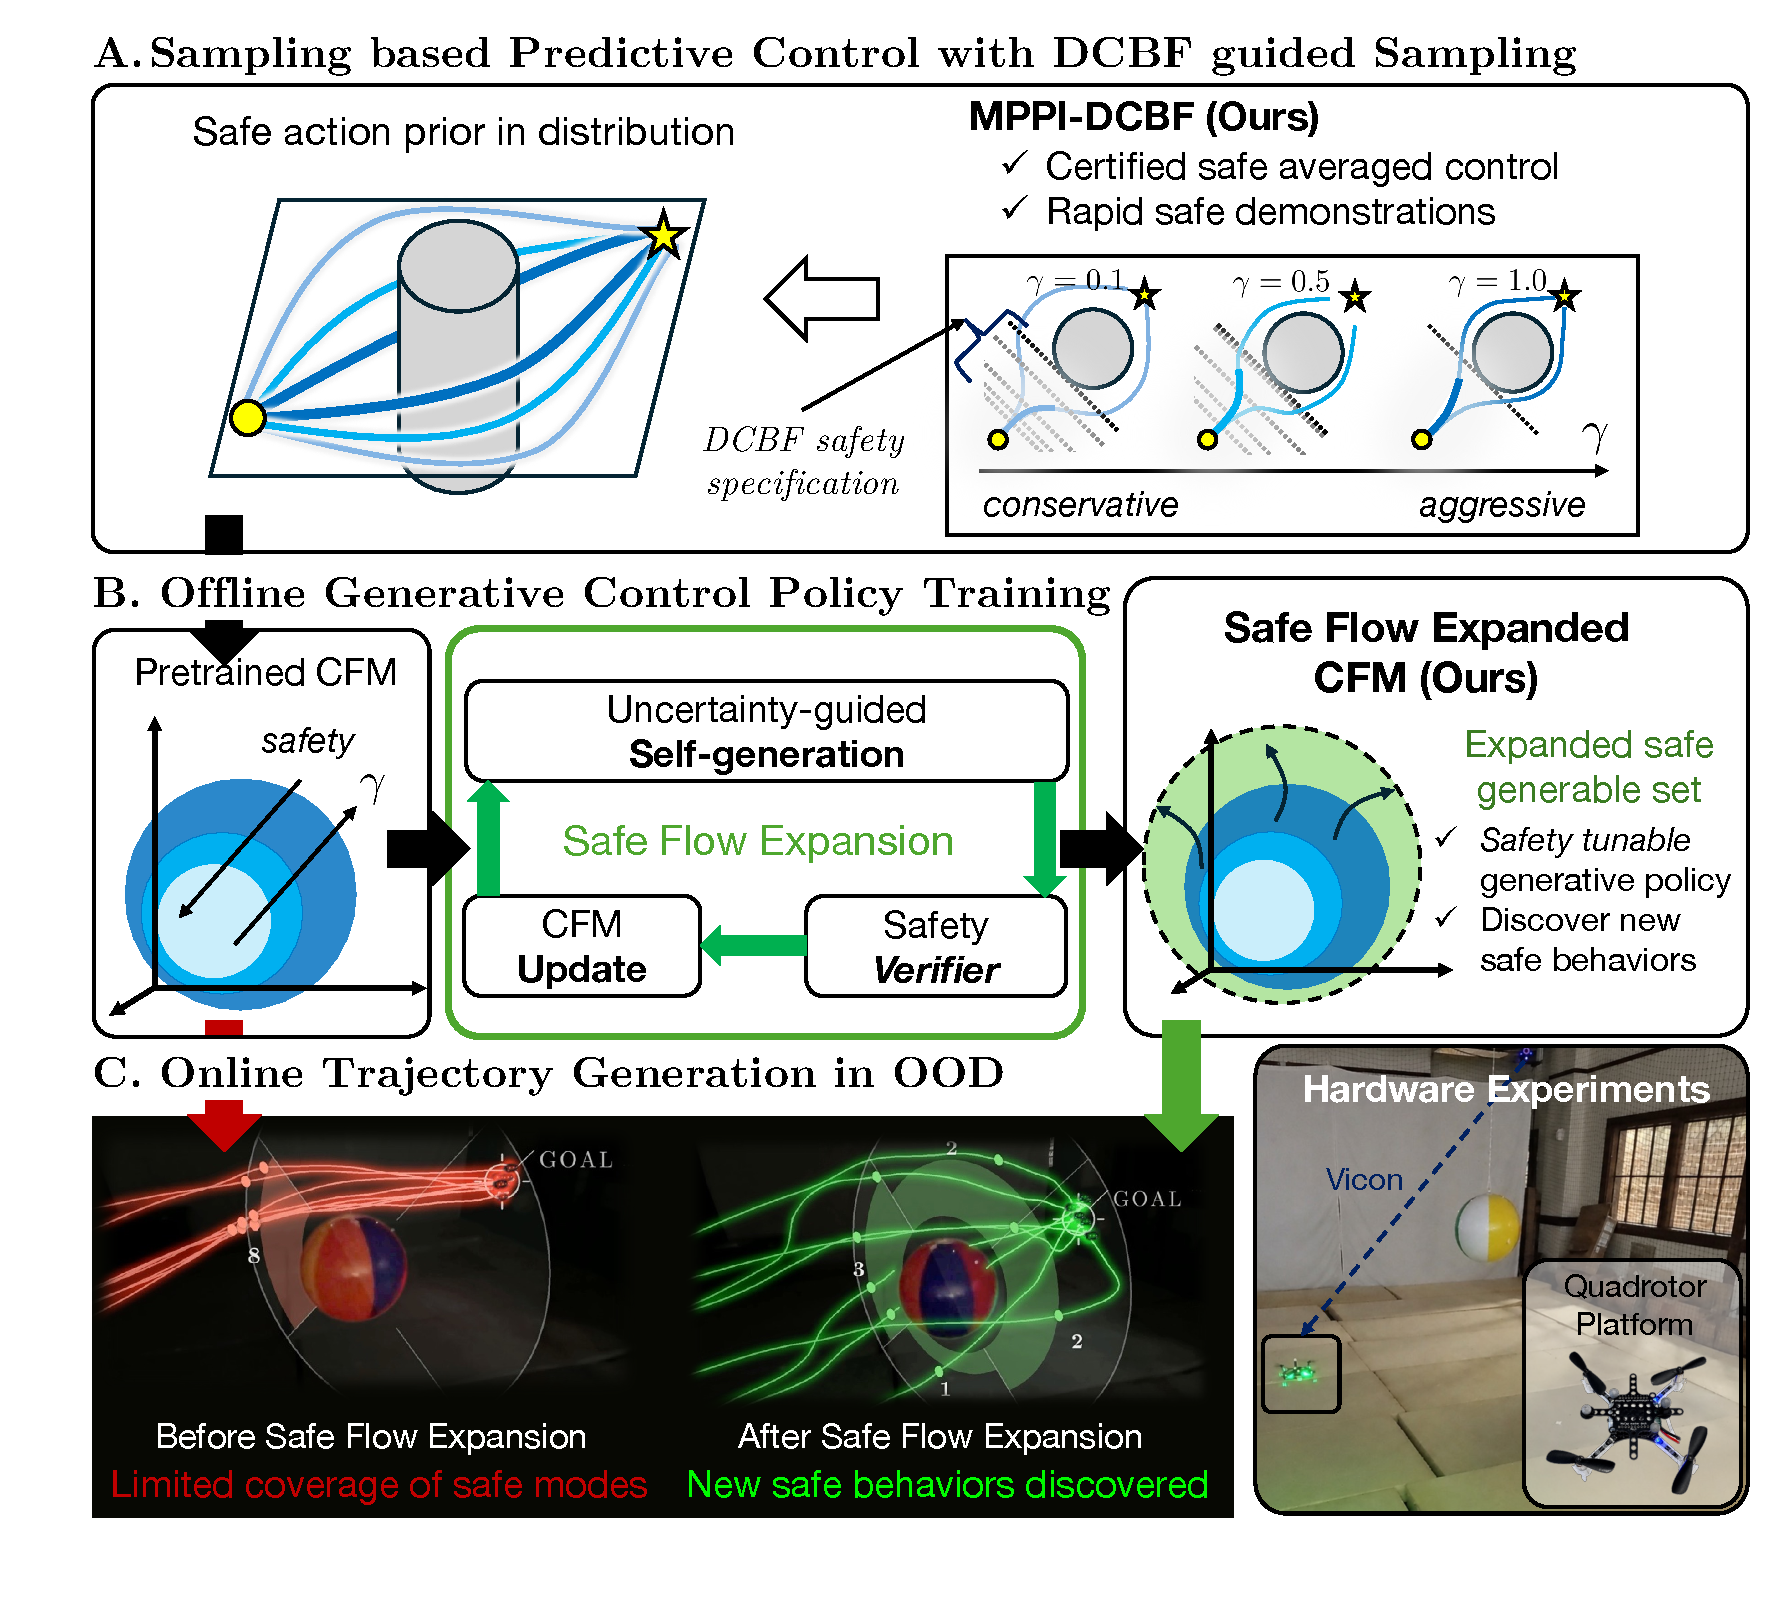
\includegraphics[width=\linewidth]{images/sfe_v3.pdf}
    \vskip -0.1 true in
    \caption{
    Overview of the proposed framework for planning in previously unseen environments. (A) MPPI-DCBF generates demonstrations conditioned on safety parameter $\gamma$. (B) SFE self-generates actions, verifies them, and updates the CFM policy offline. (C) The expanded policy discovers new safe modes in OOD environments, demonstrated on a Crazyflie quadrotor.
    }
    \vskip -0.3 true in
    \label{fig:hero}
\end{figure}

In this work, we use a multi-step safety certificate for  online rollout sampling in SBPC and action generation by a CFM policy,
%can benefit from a multi-step safety certificate 
as an alternative to optimization-based safety filters. Across different motion planning problems, we restrict the predicted action sequences to \emph{valid} actions that satisfy a finite-horizon discrete-time CBF (DCBF) condition, which includes a pointwise safety condition as its first step. Practically, we require the online planner to be computationally light and the generative policy to produce valid and diverse priors even in OOD scenarios. 

\textbf{Contributions.} MPPI and CFM policies share a sampling-based structure, which can be used to train CFM policies on demonstraions from SPBC \cite{Kurtz_GPC}. In this paper, we show how this structure can incorporate explicit safety conditions on both sides, enforcing safety constraints in motion planning for both online MPPI and pretrained CFM policies. This new analysis allows us to adapt active flow expansion~\cite{de2026active} to address distribution shift, improving the CFM policy's coverage of valid actions while also maintaining safety. Because a single parameter $\gamma$ modulates our safety constraint and conditions the CFM policy, our framework has the extra benefit of tunable safety at inference time.

Our key contributions are as follows: \textbf{(i)} 
We introduce \emph{MPPI-DCBF}, which certifies safety against MPPI's averaging process by restricting rollouts to a common convex polytope, with modest computational overhead compared to vanilla MPPI.
% This approach provides single-step safety certification under nonlinear control-affine dynamics and the entire predicted horizon for LTI systems. 
Establishing recursive feasibility remains future work, as with MPC-CBF~\cite{zeng2021safety,zeng2021enhancing}.
% MPPI-DCBF requires only $25\%$ more computation than vanilla MPPI. 
\textbf{(ii)}  
We leverage these insights to introduce {\em Safe Flow Expansion} (SFE) for CFM policies.
% When the policy must operate in conditions that are OOD from its training data, 
% SFE self-generates actions with uncertainty guidance, verifies them under the same finite-horizon DCBF conditions, and continues pretraining on valid actions to expand the \emph{generable set}~\cite{de2026active}.
SFE improves action validity and discovers new safe modes in OOD environments using only one generated action per replanning step.
\textbf{(iii)} 
We evaluate the framework in 2D cluttered and pedestrian environments and on a 3D quadrotor, in simulation and on hardware, and we show MPPI-DCBF on a 7-DoF manipulator among non-convex obstacles.
% The remainder of this paper is organized as follows...
% Under the stated assumptions, we connect MPPI-DCBF demonstrations to an initial safe set for SFE's expansion analysis
% and derive a lower bound on the probability that a generated batch contains a valid action at a fixed context and $\gamma$.
% We further evaluate how $\gamma$ and generated batch size trade off safety and performance.

\section{Preliminaries}
We study discrete-time dynamical systems of the form
\begin{equation}
\x_{k+1}=f(\x_k)+g(\x_k)\u_k,
\label{eq:dynamical_system}
\end{equation}
where $f,g$ are continuous, $k\in\mathbb Z$, and $\x_k\in\mathcal X\subseteq\mathbb R^{n_x}$ and $\u_k\in\mathcal U\subseteq\mathbb R^{n_u}$ denote the state and control input at step $k$, respectively. At each sampling time $t_k$, the controller plans the inputs $\{\u_{k+i}\}_{i=0}^{H-1}$ and predicts states $\{\x_{k+i}\}_{i=1}^{H}$, with $t_{k+i}=t_k+i\Delta t$ for a fixed sampling interval $\Delta t$.

% \vspace{-2.0mm}
\subsection{Model Predictive Path Integral control}
For control system~\eqref{eq:dynamical_system}, MPPI optimizes a mean control sequence in a convex admissible set $\mathcal U$ over horizon $H$ by sampling and cost-based reweighting~\cite{williams2016aggressive}.
It samples $M$ candidate sequences $\mathbf u^{(m)}_{k+i}=\bar{\mathbf u}_{k+i}+\varepsilon^{(m)}_{k+i}$ around the previous solution shifted one step $\bar{\mathbf u}_{k+i}$ to warm-start the optimization, where $\varepsilon^{(m)}_{k+i}\sim\mathcal N(0,\Sigma)$, for $m=1,\ldots,M$.
Each candidate is rolled out from $\x_k$ using~\eqref{eq:dynamical_system} to evaluate its cost
\begin{equation}
\setlength{\jot}{0pt}
S^{(m)}\!=\!\phi\bigl(\mathbf{x}^{(m)}_{k+H}\bigr)
\!+\!\!\sum_{i=0}^{H-1}\Big(\!q\,\!\bigl(\mathbf{x}^{(m)}_{k+i}\bigr)
\!+\!\tfrac{1}{2}\,\mathbf{u}^{(m)\top}_{k+i}R\,\mathbf{u}^{(m)}_{k+i}\Big),
\label{eq:mppicost}
\end{equation}
where $q$ and $\phi$ are the stage and terminal state costs, $R\in\mathbb R^{n_u\times n_u}$ is the control weight, and $\Sigma$ is the sampling covariance.
MPPI then optimizes a mean control sequence using weights $\omega_m=\exp(-(S^{(m)}-S_{\min})/\lambda)$, where $S_{\min}=\min_\ell S^{(\ell)}$ and $\lambda>0$ is the temperature:
\begin{equation}
\mathbf u^\star_{k+i}
=
\frac{\sum_{m=1}^{M}\omega_m\mathbf u^{(m)}_{k+i}}
     {\sum_{m=1}^{M}\omega_m},
\quad i=0,\ldots,H-1.
\label{eq:mppi-update}
\end{equation}
Only the first control $\uk^\star$ is applied before replanning.
%This parallelizable sampling process is well-suited to solving non-convex optimal control problems on GPU hardware. However, a key challenge arises in safety-critical applications. 
Prior work incorporates safety through the cost function~\cite{williams2016aggressive}, with gradient-based optimization~\cite{yin2023shield}, or by executing the lowest-cost candidate sequences under a CBF filter~\cite{rabiee2024guaranteed}. 
% TODO introduce averaging issue here? or later?
While these methods can be practical, they do not address that MPPI during the convex averaging process~\eqref{eq:mppi-update} can achieve a formal safety certificate. 

\subsection{Discrete-Time Control Barrier Functions}
Let \(\mathcal{C}=\{\x\!\in\!\mathbb{R}^{n_x}\!:\!h(\x)\!\ge\!0\}\) denote the \emph{safe set} for a continuous $h$.
A function $h$ is a DCBF
for~\eqref{eq:dynamical_system} if there exists $\gamma\in(0,1]$
such that, for every $\x_k\in\mathcal C$, there exists
$\u_k\in\mathcal U$ satisfying
\begin{equation}
    \Delta h(\x_k,\u_k)\;:=\;h(\x_{k+1})-h(\x_k)\;\ge\;-\gamma\,h(\x_k).
    \label{eq:dtcbf}
\end{equation}
If $\x_0\in\mathcal C$ and \eqref{eq:dtcbf} holds
at every step, then \(h(\x_k)\!\ge\!(1-\gamma)^{k}\,h(\x_0)\), so the fixed set $\mathcal{C}$ is forward invariant~\cite{ames2014cbf,agrawal2017discrete}.

Our safety specification is obstacle avoidance. We first model the robot as a point $\q=\piq(\x)$,
where $\piq:\mathbb R^{n_x}\to\mathbb R^d$ is a linear projection that maps the robot state to position. 
Let $\mathcal I(\xk)\subset\mathbb N$ index the convex obstacles observed at $\xk$.
For each $j\in\mathcal I(\xk)$, let $\p_j$ be its closest  point to $\qk$ and $\n_j$ its outward unit normal. Assume \(\n_j^\top(\qk-\p_j)>0\), define
\begin{equation}
h_j^{\mathrm{aff}}(\x;\xk) :=\n_j^\top(\q-\p_j)/\n_j^\top(\q_{k}-\mathbf{p_j}).
\label{eq:aff_barrier}
\end{equation}
For the DCBF constraint used for MPPI safety, we use its pointwise minimum as the ego-centric safety function
\begin{equation}\label{eq:poly_single}
h^{\mathrm{poly}}(\x;\xk):=\min_{j\in\mathcal I(\xk)} h_j^{\mathrm{aff}}(\x;\xk).
\end{equation}
The obstacle-free half-spaces bounded by the supporting hyperplanes define the nominal polytope for MPPI safety:
\begin{equation}
\mathcal P^{\mathrm{nom}}(\xk)
:=\bigcap_{j\in\mathcal I(\xk)}
\left\{
\q\in\mathbb R^d:
\n_j^\top(\q-\p_j)\ge0
\right\}.
\label{eq:nominalpolytope}
\end{equation}
Accordingly, the safe set for each horizon $i$ is defined as
\begin{equation}
\mathcal C_i^{\mathrm{poly}}
:=
\left\{
\x\in\mathbb R^{n_x}
\mid
h^{\mathrm{poly}}(\x;\xk)\ge(1-\gamma)^i
\right\}.
\label{eq:poly_safeset}
\end{equation}
Each $\mathcal C_i^{\mathrm{poly}}$ is convex, and since
$(1-\gamma)^i\ge0$, every $\x\in\mathcal C_i^{\mathrm{poly}}$
satisfies $\piq(\x)\in\mathcal P^{\mathrm{nom}}(\xk)$.

\subsection{Conditional Flow Matching for policy learning}
% CFM policies learn to map noise and observations to action sequences through supervised learning~\cite{Kurtz_GPC,mizuta2025unified}.
CFM is increasingly used for robotic trajectory and policy generation \cite{Kurtz_GPC,mizuta2025unified}.
Policy generation learns a mapping from noise to entire action sequences via end-to-end supervised learning.
% but it can struggle to generalize to OOD environments, where it may require complete retraining \cite{ye2024efficient}. 
We train CFM policies on MPPI-DCBF expert action sequences (hereafter, an \emph{action}). Let $\hat{\mathbf u}^{\star}$ denote the optimized control sequence~\eqref{eq:mppi-update}, and set
$\z:=\hat{\mathbf u}^{\star}$. 

Concretely, for a fixed observation and safety parameter \((\o,\gamma)\), let $p_1^\theta(\cdot\mid\o,\gamma)$ denote the model density at terminal flow time $t=1$.
The CFM model is trained to sample from the unknown distribution of $\z$ conditioned on \((\o,\gamma)\).
During training, we sample $(\z,\o,\gamma)\sim p_{\mathrm{data}}$, $\epsilon\sim\mathcal N(0,I_{n_z})$, and $t\sim\mathrm{Unif}[0,1]$, where $n_z=Hn_u$.
We use an optimal transport conditional probability path $\x_t\!=\!(1-t)\epsilon+t\z$, whose velocity is $\dot{\x}_t=\z-\epsilon$~\cite{lipman2022flow}. 
The CFM objective is
\begin{equation}
\mathcal{L}(\theta)=
\mathbb{E}_{
% \substack{
% t\sim\mathrm{Unif}[0,1],\\
% \epsilon\sim\mathcal{N}(0,I_{n_z}),\\
% (\z,\o,\gamma)\sim p_{\mathrm{data}}
% }
}\!
\left[
\left\|
\mathbf v_t^\theta(\x_t\mid\o,\gamma)-(\z-\epsilon)
\right\|^2
\right].
\label{eq:cfm-loss}
\end{equation}
At inference, an action is generated by integrating 
$\dot{\x}_t=\mathbf v_t^\theta(\x_t\!\mid\!\o,\gamma)$
from $\x_0\sim\mathcal N(0,I_{n_z})$ to $t=1$, from which the first control is executed in receding horizon fashion.

\subsection{Generable Set Expansion}
% Pretrained generative policies can be improved through reward-based fine-tuning~\cite{domingo2025adjoint} without expensive expert demonstrations. 
Active Flow Expansion~\cite{de2026active} is a recent active learning framework for generative models. Under proper conditions, it enlarges the \textit{$\tau$-generable set} \(\Omega^\tau_\theta\!:=\!\{\x:p_1^\theta(\x)\ge\tau\}\) of the pretrained model $\theta$ to cover a larger portion of a valid region.
Unlike reward-based fine-tuning of pretrained models~\cite{domingo2025adjoint}, its strength lies in \emph{both} increasing validity and coverage, without a specific reward term. It achieves this through iterative self-generation with uncertainty guidance and black-box verifier feedback.
In motion planning, improving both validity and coverage can lead to safer and more diverse robot behaviors. We adopt this framework to expand our pretrained CFM policy's coverage of valid actions without additional expert demonstrations.

\begin{figure}
    \centering
    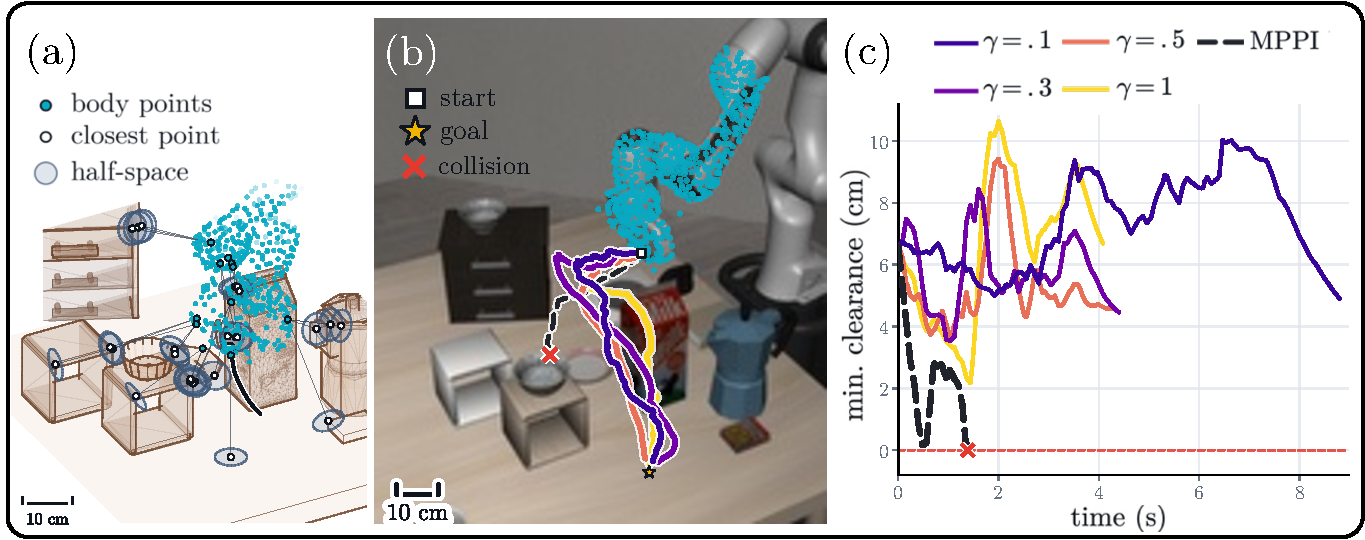
\includegraphics[width=\linewidth]{images/robotarm_v2-comp.pdf}
    \vspace{-8.0mm}
    \caption{\textbf{Simulation results of MPPI-DCBF on a Franka FR3 among non-convex objects} \textbf{(a)} Manipulator body points with their closest points and separating half-spaces of nearby convex parts, with objects modeled as multiple convex box parts. \textbf{(b)} End-effector trajectories for different $\gamma$. \textbf{(c)} Minimum clearance between the body points and the objects over time. }
    \label{fig:robotarm}
    \vskip -0.25 true in
\end{figure}

\section{Problem Definition}
\label{sec:problemdefinition}
At each replanning step $k$, let $J(\hat{\mathbf u};\x_k)$ denote the cost of the nominal rollout by the control $\hat{\mathbf u}$ from $\x_k$, using the stage and terminal costs in~\eqref{eq:mppicost}. 
We use an ego-centric safety function $h(\cdot;\x_k)$, whose nonnegative superlevel set lies in free space and which satisfies $h(\x_k;\x_k)=1$.
In our method, MPPI uses a common safety function for all sampled rollouts, while SFE constructs one for each queried action $\hat \u$.
We formulate safe planning as
\begin{subequations}
\setlength{\jot}{1pt}
\label{eq:problemdef}
\begin{align}
& &&\min_{\hat{\mathbf u}\in\mathcal U^H}\quad
J(\hat{\mathbf u};\x_k)\\
& \text{s.t.}\;
&& \text{dynamics~\eqref{eq:dynamical_system} at steps } k,\ldots,k+H-1,\\
&&&
\x_{k+i}\in\mathcal X,
\; i=0,\ldots,H,\\
&&& h(\x_{k+i};\x_k)\ge(1-\gamma)^i,
\; i=1,\ldots,H.
\label{eq:poly}
\end{align}
\end{subequations}
% TODO: We instead use a common convex inner approximation to guarantee the safety of the MPPI control after weighted averaging, as established below.
Direct optimization with a non-convex $h$ does not generally guarantee recursive feasibility for this problem and often makes real-time implementation computationally intractable~\cite{rawlings2020model}.
We address the safety constraint~\eqref{eq:poly} by constructing safety functions that define a convex inner approximation of the free space suited to online planning and offline policy expansion. 

In particular, the \emph{nominal} and \emph{verifier} polytopes in the following section define safety functions whose superlevel sets specify the finite-horizon DCBF constraints for online MPPI and offline CFM policy expansion, respectively.
In both cases, $h$ is constructed from $\xk$ and the observed obstacle $\mathcal I(\xk)$ and is fixed over the prediction horizon $i=1,\cdots,H$.
The bounds $(1-\gamma)^i$ derive from the finite-horizon DCBF condition, with smaller $\gamma$ imposing stricter safety margins and restricting the feasible action set~\cite{zeng2021enhancing}.

\section{Method}
\subsection{MPPI-DCBF}
We propose MPPI with DCBF-based sample rejection (MPPI-DCBF), which accepts only rollouts satisfying the safety specification~\eqref{eq:poly} with $h=h^\text{poly}$ in ~\eqref{eq:poly_single} and uses their control sequences in the weighted update~\eqref{eq:mppi-update}. The following results require at least one accepted rollout, with all corresponding control inputs lying in the convex admissible set $\mathcal U$. Let $\hat\omega_m\ge0$ denote the normalized MPPI weights over accepted rollouts, with $\sum_m\hat\omega_m=1$.
\begin{proposition}
\label{prop:1}
For the system~\eqref{eq:dynamical_system}, if every accepted rollout satisfies
$\x^{(m)}_{k+1}\in\mathcal C_1^{\mathrm{poly}}$,
then the MPPI control computation process produces
$\x^\star_{k+1}\in\mathcal C_1^{\mathrm{poly}}$.
\end{proposition}
For linear time-invariant (LTI) dynamics,
\begin{equation}
\x_{k+1}=A\x_k+B\u_k,
\label{eq:lti}
\end{equation}
the certificate extends to the entire predicted horizon.
\begin{proposition}
\label{prop:2}
For the LTI system~\eqref{eq:lti}, if every accepted rollout satisfies
$\x^{(m)}_{k+i}\in\mathcal C_i^{\mathrm{poly}}$
for $i=1,\ldots,H$, then the MPPI control produces
$\x^\star_{k+i}\in\mathcal C_i^{\mathrm{poly}}$
for every $i=1,\ldots,H$.
\end{proposition}
\emph{Proof of Propositions~\ref{prop:1} and~\ref{prop:2}.} Since all rollouts start at $\x_k$, control-affine dynamics give $\x^\star_{k+1}=\sum_m\hat\omega_m\x^{(m)}_{k+1}$.
For LTI dynamics, induction gives $\x^\star_{k+i}=\sum_m\hat\omega_m\x^{(m)}_{k+i}$ throughout the horizon. Both claims follow from convexity of $\mathcal C_i^{\mathrm{poly}}$.\hfill$\blacksquare$

Thus, the common convex safe sets preserve safety under MPPI averaging for the executed step of~\eqref{eq:dynamical_system} and the full predicted horizon of~\eqref{eq:lti}. These guarantees assume the existence of accepted controls that satisfy the DCBF constraint~\eqref{eq:poly} with $h=h^\text{poly}$ but do not establish recursive feasibility. A similar distinction for MPC-CBF likewise does not ensure recursive feasibility, as discussed in~\cite[Remark~1]{zeng2021enhancing}.

\noindent\textbf{Extension: Multi-Body Points and Nonconvex Obstacles.} The affine-barrier construction in~\eqref{eq:aff_barrier} assumed a point robot $\q=\pi_q(\x)$ and applies to general convex obstacles, as is common in safety-critical planning~\cite{agrawal2017discrete, mizuta2025unified}.
MPPI-DCBF can be extended to more general motion planning problems with nonconvex obstacles that can be represented as a union of convex sets~\cite{zhang2020optimization,mjx}.
To account for robot geometry, we also construct the safety function at multiple body points~\cite{wilkinson2026full}. Let $\pi_c$ map the state to a body point $\q^{(c)}=\pi_c(\x)$, with body Jacobian $J_c=\partial \pi_c/\partial \x \in \mathbb R^{3\times n_x}$. For each of the $N_c$ sampled body points, the linearization of $\pi_c$ at $\xk$ is
\begin{equation}
\tilde{\pi}_c(\x;\xk)
:=\pi_c(\xk)+J_c(\xk)(\x-\xk).
\end{equation}
Each pair of a linearized body point $\tilde{\pi}_c(\x;\xk)$ and a convex obstacle part $\mathcal O_j$ defines an affine barrier function $h^{\mathrm{aff}}_{c,j}$ via~\eqref{eq:aff_barrier}. The safety function~\eqref{eq:poly_single} can be extended as
\begin{equation}
h^{\mathrm{poly}}(\x;\xk)
:=\min_{1\le c\le N_c}\min_{j\in\mathcal I(\xk)}
h^{\mathrm{aff}}_{c,j}(\x;\xk).
\label{eq:poly_multi}
\end{equation}
Taking the minimum of these affine functions preserves convexity of the safe sets, so Proposition~\ref{prop:2} applies to the linearized body points under its stated dynamics conditions. 
%Our setup for circular obstacles with a single body point is recovered with $N_c=1, \pi_c=\pi_q$.

Fig.~\ref{fig:robotarm} shows MPPI-DCBF on a Franka FR3 arm, a seven degree of freedom (7-DOF) arm, in \emph{LIBERO}~\cite{liu2023libero}.
% ~\footnote{We omit a 3-D visualization of the level sets of~\eqref{eq:poly_multi}, which are defined in the high-dimensional configuration space through constraints on multiple body points. The 7-DoF Franka FR3 has one redundant degree of freedom, so different configurations with the same task-space pose can yield different safety function values.}.
We use $N_c=559$ body points, $\Delta t=0.08$s, $H=10$. 
All MPPI-DCBF trajectories reach the goal without collision. $\gamma=0.1$ achieves the largest minimum clearance but takes the longest to reach the goal. 
%Whereas the MPPI baseline without sample rejection collides with an object. 
% TODO: Is this needed?: For the subsequent formal analysis, we return to the original point-robot setting.

% Every MPPI-DCBF trajectory reaches the goal without collision for all tested $\gamma$, and the minimum clearance was largest at $\gamma=0.1$. For the following sections, we return to the original settings for the formal analysis.
%We omit a 3-D visualization of the levelsets of~\eqref{eq:poly_multi} because, for a Franka FR3 it has an extra degrees of freedom so for the $\x$ there are many possible $\q$ which affects the affine function for each sampled points, thus the safe set is defined by constraints on multiple body points in the robot’s high-dimensional configuration space and cannot be represented in 3-D position space.

\subsection{Multi-step Safety Verification}

\begin{figure}[!t]
\centering
    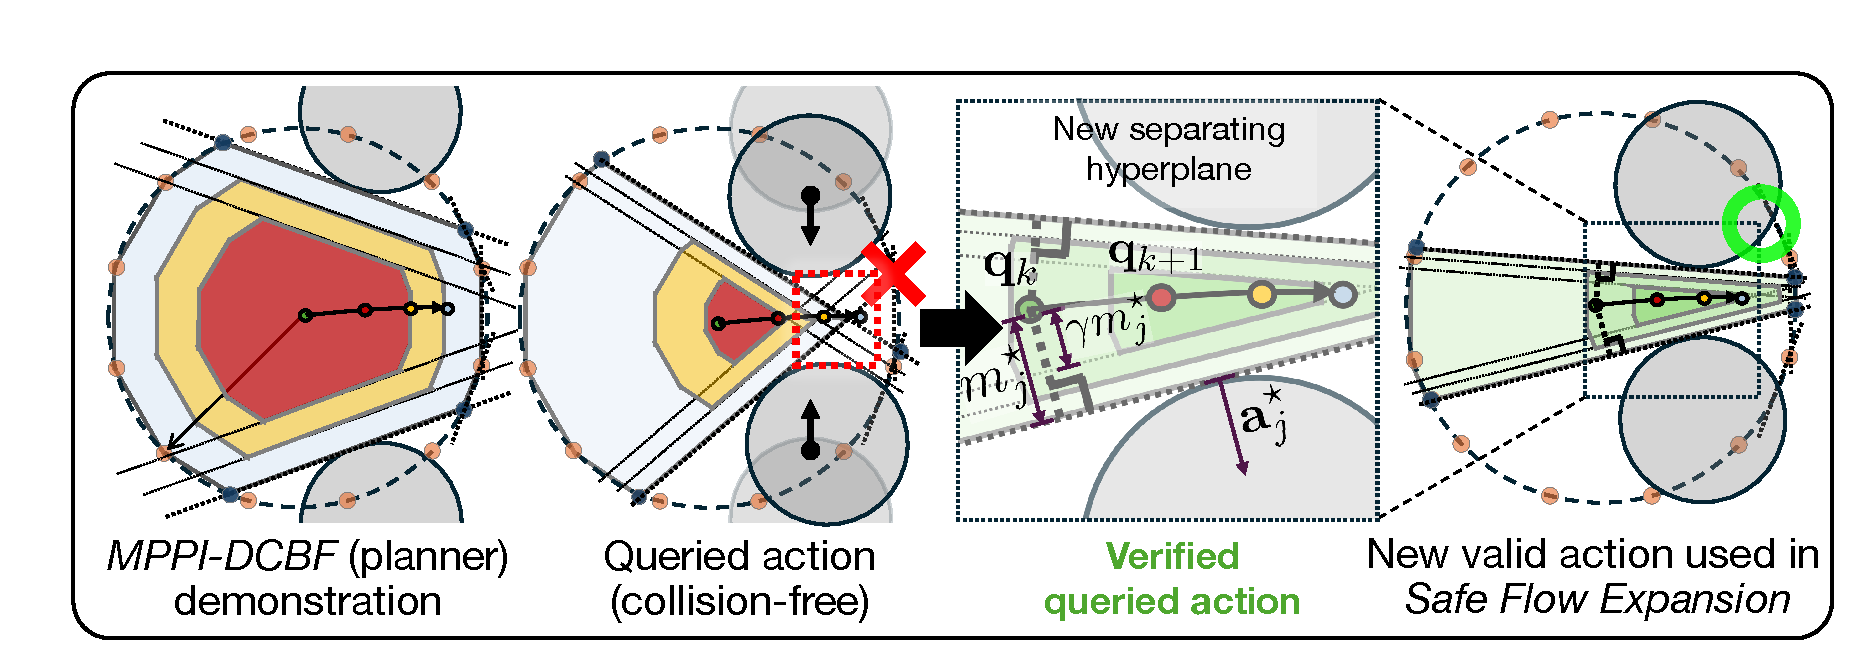
\includegraphics[width=1.0\linewidth]{images/pedestrian_v1_illustrative.pdf}
    \vspace{-7.0mm}
    \caption{Illustrative example of MPPI-DCBF demonstration using nominal polytope \eqref{eq:poly_safeset} and SFE verification using verifier polytope~\eqref{eq:verifierpolytope} \( (H=3, d=2, \mathcal I(\xk) = \{1,2\}, \gamma=0.5) \). The verifier admits collision-free queried actions that the nominal polytope excluded.
    }
\label{fig:illustration}
\vskip -0.3 true in
\end{figure}

We now turn to expand the generative policy beyond the MPPI-DCBF demonstrations. In nonconvex free space, the nominal polytope~\eqref{eq:nominalpolytope} may exclude collision-free rollouts in other modes~\cite{deits2015computing}. We therefore define a verifier that searches for separating half-spaces around each queried action to certify the same finite-horizon safety specification~\eqref{eq:poly}.

For a queried action $\hat{\mathbf u}$, let $\x_{k+i},i\!=\!0,\!\ldots\!,H$, denote the resulting predicted states. For each convex configuration-space obstacle \(j\!\in\!\mathcal I(\xk)\), represented as \(\mathcal O_j\!:=\!\{\q\!\in\!\mathbb R^d\!:\!\|\q\!-\!\oj\|_2\!\le\! r_j\},\)
the verifier constructs a separating half-space \(\mathbf a_j^\top(\mathbf q-\qk)\le m_j,\)
by solving the maximization problem
\noindent
\begin{align}
\max_{\aj,m_j}\ & m_j \label{eq:socp}\\
\text{s.t. }\ &
\aj^\top(\qki-\qk)\le\big(1-(1-\gamma)^i\big)m_j
\; (i=1,\dots,H), \notag\\
& r_j\|\aj\|_2\le \aj^\top(\oj-\qk)-m_j, \notag\\
& \|\aj\|_2\le1,\quad 0<m_{\min}\le m_j, \notag
\end{align}
Problem~\eqref{eq:socp} is a second-order cone program (SOCP), solved with Clarabel through CVXPY~\cite{goulart2026clarabel}. Specifically, the first trajectory constraint imposes the safety specification in \eqref{eq:poly} with \(h(\xki;\xk)=1-\aj^\top(\qki-\qk)/m_j\) equal to 1 at the current position and is required to remain at least $(1-\gamma)^i$. The separation constraint follows from
\[
\inf_{\q\in\mathcal O_j}\aj^\top(\q-\qk)
=
\aj^\top(\oj-\qk)-r_j\|\aj\|_2
\ge m_j.
\]

\begin{figure}[t]
    \centering
    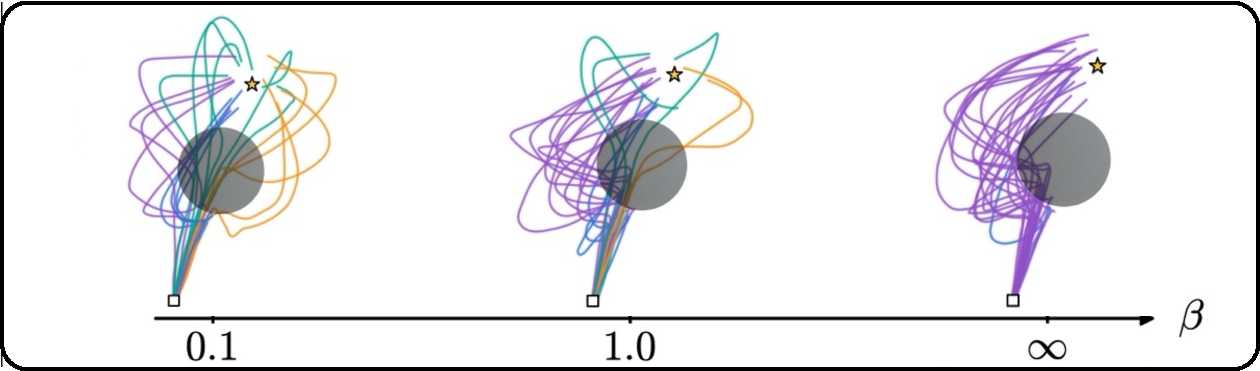
\includegraphics[width=\linewidth]{images/beta_v3-comp.pdf}
    \vspace{-7.0mm}
    \caption{Rollouts of the expanded policy in the 3D single sphere task after SFE, run with the same parameters for expansion but for $\beta=0.1$, $\beta=1.0$, and $\beta\to\infty$ (standard sampling at the current policy, $\hat{\mathbf u} \sim p_1^{\theta_n}$). Colors show the four modes: above, below, left, and right. Smaller $\beta$ puts more weight on uncertain actions and discovers new trajectories.}
    \label{fig:beta}
    \vskip -0.3 true in
\end{figure}

The remaining constraints fix the scale of the normal and impose the strictly positive margin $m_{\min}\!>\!0$. With $(\aj^\star,m_j^\star)$ a solution for obstacle $j$. The resulting verifier polytope for a queried action is (See Fig.~\ref{fig:illustration} for illustration) 
\begin{equation}
\mathcal P(\hat{\mathbf u};\o,\gamma):=\nspace{-10}\bigcap_{j\in\mathcal I(\xk)}\nspace{-10}\{
\q\in\mathbb R^d:
{\aj^\star}^{\!\top}(\q-\qk)\le m_j^\star\}.
\label{eq:verifierpolytope}
\end{equation}
In practice, we augment both the nominal and verifier polytope constructions with auxiliary half-spaces that bound the sensing region so that $\mathcal P$ is bounded (\textit{e.g.,} 12 orange points in Fig.~\ref{fig:illustration} form such half-spaces).
Now we describe the important concept of the objective of proposed algorithm, Safe Flow Expansion, \textit{validity} of a queried action.

\begin{definition}
\label{def:verifier}
Let \(v_\gamma(\hat{\mathbf u};\o) \in \{0, 1\}\) be an indicator function that equals $1$ if and only if~\eqref{eq:socp} is feasible for \emph{every} $j\in\mathcal I(\xk)$ at action $\hat{\mathbf u}$, context $\o$, and safety parameter $\gamma$.
The \textit{valid action set} is defined as
\begin{equation}
    \Omega^\star(\o,\gamma)
    :=
    \left\{
    \hat{\mathbf u}\in\mathcal U^H:
    v_\gamma(\hat{\mathbf u};\o)=1
    \right\},
    \label{eq:verifier-certified-set}
\end{equation}
and action \(\hat{\mathbf u} \in \Omega^\star(\o,\gamma)\) is a \textit{valid} action that guarantees the existence of a verifier polytope~\eqref{eq:verifierpolytope}.
\end{definition}

The following result connects this deterministic notion of validity to the MPPI-DCBF demonstrations.

\begin{proposition}
\label{prop:nominal-verifier}
Let $\p_j$ and the
outward unit normal $\n_j$ define the nominal face, and let \(d_j:=\n_j^\top(\qk-\p_j)=\|\qk-\oj\|_2-r_j>0.\)
If $m_{\min}\le\min_{j\in\mathcal I(\xk)}d_j$, then, for every
$\hat{\mathbf u}\in\mathcal U^H$ whose resulting trajectory satisfies
\[
h^{\mathrm{poly}}(\xki;\xk)\ge(1-\gamma)^i,
\quad i=1,\ldots,H,
\]
the choice $(\aj,m_j)=(-\n_j,d_j)$ is feasible
for~\eqref{eq:socp}, and hence
$\hat{\mathbf u}\in\Omega^\star(\o,\gamma)$.
\end{proposition}

Under the conditions of Proposition~\ref{prop:nominal-verifier}, the averaged action from MPPI-DCBF certified by Proposition~\ref{prop:2} is valid, while for a general affine system~\eqref{eq:dynamical_system}, the averaged action requires separate verification. We also note that the valid actions with desired safety level $\gamma$ have the following property.

\begin{proposition}
\label{prop:gamma-effect}
For any $\o$ and
$0<\gamma_1\le\gamma_2\le1$,
\setlength{\abovedisplayskip}{2pt}
\setlength{\abovedisplayshortskip}{2pt}
\begin{equation}
\Omega^\star(\o,\gamma_1)
\subseteq
\Omega^\star(\o,\gamma_2).
\end{equation}
\end{proposition}
\noindent\emph{Proof.}
For every horizon $i$,
$1-(1-\gamma)^i$ is nondecreasing in $\gamma$.
Thus, any valid action at $\gamma_1$ also satisfies the trajectory constraints at $\gamma_2$, no other constraint of~\eqref{eq:socp} involves $\gamma$. \hfill$\blacksquare$

We seek to generate valid actions at the desired safety level $\gamma$, despite the tighter validity requirements at smaller $\gamma$ (\Cref{prop:gamma-effect}). We start by pretraining the CFM policy on a finite set of valid MPPI-DCBF demonstrations.
\SetAlgoSkip{}
\begin{algorithm}[t]
\caption{Safe Flow Expansion}
\label{alg:sfe}
\small
\LinesNumbered
\DontPrintSemicolon
\KwIn{pretrained CFM $\theta_0$; verifier $v_{\gamma_k}$; dynamics $f,g$;
execution cost $C$; rounds $N$; success target $P$;
proposal and verification budgets $K\ge B$}
\KwOut{expanded CFM $\theta_N$}
$\mathcal B_0\gets\varnothing$\;
\For{$n\gets0$ \KwTo $N-1$}{
$\sigma_n\gets\textsc{UpdateUncertainty}(\mathcal B_n)$;\quad
$\mathcal D_n,\mathcal S_n\gets\varnothing$\;
\Repeat{$|\mathcal S_n|\ge P$}{
rollout $\theta_n$ in parallel\;
\ForEach{replanning step $k$ with context $(\o_k,\gamma_k)$}{
draw $\hat{\mathbf u}^{(1:B)}$ from $K$ proposals
by~\eqref{eq:importancesampling}\;
$y_j\gets v_{\gamma_k}(\hat{\mathbf u}^{(j)};\o_k)$,
$\;\mathcal J_k^+\gets\{j:y_j=1\}$\;
$\mathcal D_n\gets\mathcal D_n\cup
\{(\o_k,\gamma_k,\hat{\mathbf u}^{(j)},y_j)\}_{j=1}^{B}$\;
\lIf{$\mathcal J_k^+=\varnothing$}{\textsc{RestartRollout}()}
$j^\star\gets\arg\min_{j\in\mathcal J_k^+}
C(\o_k,\hat{\mathbf u}^{(j)})$\;
$\mathbf u_k\gets[\hat{\mathbf u}^{(j^\star)}]_0$,
$\;\mathbf x_{k+1}\gets f(\xk)+g(\xk)\uk$\;
}
add every restart-free rollout to $\mathcal S_n$\;
}
$\mathcal B_{n+1}\gets\textsc{UpdateBuffer}(\mathcal B_n,\mathcal D_n)$;\quad

$\theta_{n+1}\gets\textsc{UpdateCFM}(\theta_n,\mathcal D_n^{+})$\;
}
\Return{$\theta_N$}\;
\end{algorithm}

\subsection{Safe Flow Expansion (SFE)}
With the pretrained CFM policy, we now introduce Safe Flow Expansion (Alg.~\ref{alg:sfe}) to iteratively sample actions with uncertainty guidance and update the CFM policy to acquire safe valid actions absent from the demonstrations, including those excluded by MPPI-DCBF's shared nominal polytope. 
The policy \(\theta_n\) at round $n$ induces the \textit{conditional generable set} associated with the  density lower bound \(\tau\) defined as:
\begin{equation}
    \Omega_{\theta_n}^{\tau}(\o,\gamma)
    :=\{
    \hat{\mathbf u}\in\mathcal U^H:
    p_1^{\theta_n}(\hat{\mathbf u}\mid\o,\gamma)\ge\tau
    \},
    \label{eq:conditional-generable-set}
\end{equation}
Therefore, SFE aims to expand this generable set to cover a larger portion of a valid action set $\Omega^\star(\o,\gamma)$. 
% The conditional generable set contains actions to which the policy assigns density at least $\tau$. Here, we recover the pre-trained conditional generable set by setting \(n=0\).
At each iteration, Alg.~\ref{alg:sfe} samples toward actions with high uncertainty region while adhere to the current policy~\footnote{The exact Gibbs solution of
\(
p_n \in \arg\max_q \{ \mathbb{E}_q[\sigma_n(\phi_s(\hat\u))] - \beta \text{KL}(q \parallel p_1^{\theta_n})\},
\) where $\text{KL}$ denotes Kullback--Leibler divergence.}
\begin{equation}
\hat{\mathbf u}
\sim
p_1^{\theta_n}(\hat{\mathbf u}\mid\o,\gamma)
\exp\!\left(
\sigma_n\!\left(\phi_s(\hat{\mathbf u};\o,\gamma)\right)/\beta
\right)
/Z_n(\o,\gamma)
,
\label{eq:importancesampling}
\end{equation}
where $\beta\!>\!0$ is the parameter that controls the trade-off between exploration and the prior, $Z_n(\o,\gamma)$ is the normalizing constant.
% ~\footnote{Define \( Z_n(\o,\gamma)\!=\!\int_{\mathcal U^H} p_1^{\theta_n}(\mathbf u\!\mid\!\o,\!\gamma)\exp\!\left( \sigma_n\!\left(\phi_s(\mathbf u;\o,\!\gamma)\right)/\beta\right)d\mathbf u.\)}.
$\phi_s$ denotes the penultimate layer feature of the CFM vector field $\mathbf v_t^{\theta_n}(\hat \u'\!\mid\!\o,\gamma)$ evaluated at the fixed flow time $t=s$ with noised queried action $\hat \u'=s\hat\u+(1-s)\epsilon$, where $\epsilon$ is Gaussian base noise. We modeled $\sigma_n$ as the posterior standard deviation of a Gaussian process fitted on the features $\phi_s$ to the binary observations in the buffer. For $\phi=\phi_s(\hat{\mathbf u};\o,\gamma)$, define $[\mathbf K_n]_{ij}=k(\phi_i,\phi_j)$ and $[\mathbf k_n(\phi)]_i=k(\phi_i,\phi)$. The posterior standard deviation is therefore
\begin{equation}
\sigma_n(\phi)=\sqrt{k(\phi,\phi)-\mathbf k_n(\phi)^{\!\top}\left(\mathbf K_n+\nu I\right)^{-1}\mathbf k_n(\phi)},
\label{eq:gp-uncertainty}
\end{equation}
where $\nu\!>\!0$ is a regularization parameter. Intuitively, this uncertainty score is high for queried actions whose learned features are poorly represented in the queried buffer.
% At each replanning step $k$, SFE self-generates actions from the current CFM policy using the GP posterior uncertainty $\sigma_n$ in ~\eqref{eq:importancesampling} within the parallel rollouts. The verifier $v_{\gamma_k}$, defined by the finite-horizon DCBF conditions in Def.~\ref{def:verifier}, separates these queried actions $\hat{\mathbf u}^{(j)}$ into valid (\textit{i.e.,} $j\in\mathcal J_k^+$) and invalid sets, and adds both sets to $\mathcal D_n$. If no queried action is valid, the offline rollout restarts. The execution cost \(C\) ranks valid action candidates, from which the first control input of the candidate with minimum cost is executed.
% %One can set this cost as expert actions \cite{ross2011reduction} or restrict execution to a safe admissible action set \cite{alshiekh2018safe}. 
% %Even when $C$ is shared across, queried actions depend on $\gamma$ through the admissible set $\mathcal J_k^+$, thereby preserving the semantics of $\gamma$ (\textit{i.e.,} safety--performance tradeoff) through policy expansion. 
% We repeat this data acquisition until we gather $P$ successful trajectories. Both valid and invalid sets are then added to the buffer through \textsc{UpdateBuffer}, from which \textsc{UpdateUncertainty} constructs $\sigma_{n+1}$ in the next round. Finally, \textsc{UpdateCFM} uses hierarchical sampling among valid queried actions $\mathcal D_n^+ \subset \mathcal D_n$, uniformly over $\gamma$ and successful trajectories, and regresses the CFM loss~\eqref{eq:cfm-loss} on these uncertainty-guided action data. Pooling observations across contexts may make $\sigma_n$ prioritize novelty in unrelated contexts.
% We therefore use it only as an acquisition heuristic~\cite{de2026active}, while the verifier determines validity.

The verifier $v_{\gamma_k}$, defined by the finite-horizon DCBF conditions in Def.~\ref{def:verifier}, separates these queried actions $\hat{\mathbf u}^{(j)}$ into valid (\textit{i.e.,} $j\in\mathcal J_k^+$) and invalid sets, and adds both sets to $\mathcal D_n$.
The execution cost \(C\) ranks valid action candidates, from which the first control input of the candidate with minimum cost is executed.
Both valid and invalid queried actions update the uncertainty buffer after $P$ successful trajectories. If no queried action is valid, the offline rollout restarts.
\textsc{UpdateCFM} uses hierarchical sampling among valid queried actions $\mathcal D_n^+ \subset \mathcal D_n$, uniformly over $\gamma$ and successful trajectories, and regresses the CFM loss~\eqref{eq:cfm-loss} on these uncertainty-guided action data. 
Pooling observations across contexts may make $\sigma_n$ prioritize novelty in unrelated contexts. We therefore use it only as an acquisition heuristic~\cite{de2026active}, while the verifier determines validity.

\begin{figure}
    \centering
    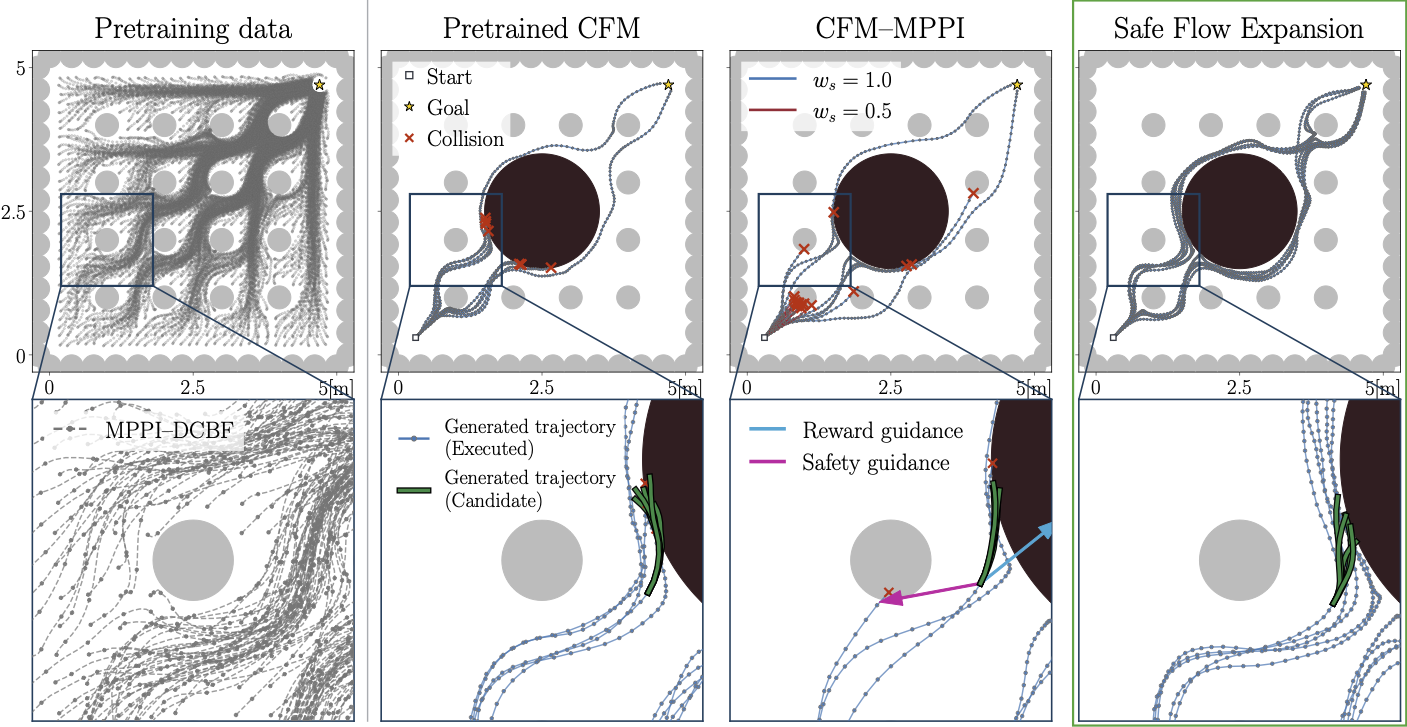
\includegraphics[width=\linewidth]{images/cluttered_rollouts_v2.png}
    % TODO change it to .pdf before submission:)
    \vspace{-7.0mm}
    \caption{SFE in an unseen giant obstacle configuration. The pretrained CFM and CFM-MPPI at two tested safety reward weights ($w_s$) are compared with SFE. After expansion, SFE learns collision-free paths around the obstacle.}
    \label{fig:2d_cluttered}
    \vskip -0.25 true in
\end{figure}

\section{Experiments and Discussion}
% ~\footnote{SFE adaptation uses the same OOD configuration for expansion and evaluation (2D cluttered and 3D single-sphere). SFE generalization evaluates on independently sampled OOD configurations unseen during expansion (2D dynamic-pedestrian and 3D cluttered).}. 
% \noindent\textbf{Evaluation protocol.}
% MPPI-DCBF generates all pretraining data under 2D and 3D double-integrator dynamics and a sampling time of $\Delta t = 0.1s$. Each of the four tasks runs three phases: in-distribution training, SFE (Alg.~\ref{alg:sfe}) in OOD environments, and final OOD testing, with start, goal, and dynamics fixed
% % ~\footnote{In \emph{SFE adaptation}, expansion and evaluation use the same OOD obstacle configuration (2D cluttered environment and 3D single-sphere environment). In \emph{SFE generalization}, evaluation uses independently sampled OOD configurations that are not used during expansion (2D dynamic-pedestrian environment and the 3D cluttered environment).}. 
% ~\footnote{SFE adaptation uses the same OOD configuration for expansion and evaluation (2D cluttered and 3D single-sphere). SFE generalization evaluates on independently sampled OOD configurations unseen during expansion (2D dynamic-pedestrian and 3D cluttered).}.
% To account for the varying difficulty of the four tasks, we use a task-specific number $P$ of successful trajectories, fixed across rounds. After each round $n$, we independently evaluate the CFM model $\theta_n$ with a 16-step ODE solver on 100 test rollouts per task and $\gamma$. 
% Data generation and training used an NVIDIA H100 NVL GPU, all online tests used an NVIDIA RTX 4060 Ti GPU.
% start \((0.3,0.3)\), goal \((4.7,4.7)\), \(5\,\mathrm{m}\times5\,\mathrm{m}\) taskspace,
% pretrained on 200k MPPI-DCBF actions of length $H$ from random initial positions to the fixed goal among regularly sized circular obstacles. Testing replaces the central obstacles with one unseen large obstacle that blocks the short demonstrated paths and requires long-horizon planning out of local minima. 
% In the \emph{2D cluttered environment}, the robot starts at \((0.3,0.3)\) and navigates toward the fixed goal at \((4.7,4.7)\) in a \(5\,\mathrm{m}\times5\,\mathrm{m}\) taskspace. The CFM model is pretrained on an MPPI-DCBF policy from a random initial position to a fixed goal position, total 200k actions of length $H$ as shown in Fig.~\ref{fig:2d_cluttered}, in a nominal environment with regularly sized circular obstacles. We tested this by replacing the central obstacles with a previously unseen large obstacle to see whether SFE can learn long-horizon, collision-free behavior and avoid getting trapped in local minima.
% We extend the social navigation setup of~\cite{mizuta2025unified} to an explicit distribution shift in crowd density and speed. Pretrained on MPPI-DCBF policy under 20 pedestrians moving at $0.5$--$1.0\,\mathrm{m/s}$, while evaluation uses 40 pedestrians moving at $1.0$--$2.0\,\mathrm{m/s}$ in independently sampled configurations not used during expansion. 
% start \((0,0)\), goal \((6,6)\), \(7\,\mathrm{m}\times7\,\mathrm{m}\) taskspace, 
% pretrained on MPPI-DCBF policy in distribution with 20 pedestrians moving at \(0.5\!-\!1.0\,\mathrm{m/s}\), whereas evaluation uses 40 pedestrians moving at \(1.0\!-\!2.0\,\mathrm{m/s}\), which demands highly reactive behavior. In these challenging dynamic tasks, the policy conditions on the 10-step history of local observations $h^\text{poly}$, unlike other tasks.
% In the \emph{2D dynamic-pedestrian environment}, the robot starts at \((0,0)\) and moves to \((6,6)\), with the simulated pedestrian environment modeled by the social force model~\cite{helbing1995social}, where each pedestrian is a modeled reactive dynamical system whose acceleration exponentially grows as agents approach. The CFM model is pretrained on an MPPI-DCBF policy in distribution with 20 pedestrians moving at \(0.5\!-\!1.0\,\mathrm{m/s}\), whereas evaluation uses 40 pedestrians moving at \(1.0\!-\!2.0\,\mathrm{m/s}\). In these challenging dynamic tasks, the policy conditions on the 10-step history of local observations $h^\text{poly}$, unlike other tasks. We tested this to capture how SFE can learn highly reactive behaviors under dynamic environments.
% 10 time steps, 32 angular bins, and 100 radial bins.
% online 3D motion planning on a \textit{Crazyflie} quadrotor. Start \((-2.5,1.5,0.9)\), goal \((0.7,-1.5,0.9)\), \(4\,\mathrm{m}\times4\,\mathrm{m}\times1.5\,\mathrm{m}\) taskspace. A Vicon motion-capture system provides quadrotor and obstacle poses at $50$ Hz. The policy replans at $10$ Hz and streams the acceleration command at $100$ Hz as the feedforward component of a full-state setpoint. Both single-sphere (Fig.~\ref{fig:hero}) and cluttered tasks (Fig.~\ref{fig:coverage}) pretrain among $4$ to $8$ randomly positioned cylinder obstacles, then test on one sphere at the start-goal midpoint or on 6 randomized spheres. The mode discovery test fixes one layout and compares the pretrained model, 5 and 10 expansion rounds, and the baseline.
% \emph{3D hardware environments}: deployed online 3D motion planning on a \textit{Crazyflie} quadrotor. The robot starts at \((-2.5,1.5,0.9)\) to \((0.7,-1.5,0.9)\) in a \(4\,\mathrm{m}\times4\,\mathrm{m}\times1.5\,\mathrm{m}\) taskspace. A Vicon motion-capture system provides quadrotor and obstacle poses at $50$ Hz. The policy replans at $10$ Hz, streaming the acceleration command at $100$ Hz as the feedforward component of a full-state setpoint.
% Additionally, in the dynamic-pedestrian task, the verifier certifies validity with respect to the currently observed obstacle geometry, frozen over the prediction horizon. We use a constant-velocity model of the pedestrians only in the execution cost to favor valid action candidates that anticipate future collisions. Consequently, avoidance of moving pedestrians beyond the frozen-scene certificate is empirical and relies on receding-horizon replanning. 
% At deployment, SFE generates \(J\) actions in parallel and 
% performs \emph{sampling}, which we refer to as mode selection by selecting the action with the lowest execution cost $C$. We use \(J=1\) by default and \(J>1\) in~\Cref{sec:tradeoff} to study its effect on safety and performance.
We evaluate SFE in two 2D simulations, a 3D quadrotor simulation, and a hardware flight experiment.
\subsection{Evaluation Protocol and Implementation}
\noindent\textbf{Evaluation protocol.}
MPPI-DCBF generates pretraining demonstrations using double-integrator dynamics with $\Delta t\!=\!0.1\mathrm{s}$. Each task comprises in-distribution pretraining, offline SFE in OOD environments, and OOD evaluation.
Each expansion round collects a task-specific number $P$ of successful trajectories. Across 3 seeds, we evaluate each checkpoint $\theta_n$ using a 16-step ODE solver on 100 rollouts per task and $\gamma$.

\noindent \textbf{Task configurations.} \emph{2D cluttered environment (Fig.~\ref{fig:2d_cluttered})}:
The policy is pretrained on 200k MPPI-DCBF actions from random starts toward a fixed goal among circular obstacles. Evaluation introduces a large central obstacle that blocks the demonstrated short routes in a $5\,\mathrm{m}\times5\,\mathrm{m}$ workspace.
\emph{2D dynamic-pedestrian (Fig.~\ref{fig:pedestrian})}:
Using the social navigation setup of~\cite{mizuta2025unified}, we pretrain the policy on MPPI-DCBF demonstrations collected among 20 pedestrians moving at $0.5$--$1.0\,\mathrm{m/s}$. Evaluation uses 40 pedestrians at $1.0$--$2.0\,\mathrm{m/s}$.
In these challenging dynamic tasks, the policy conditions on the 10-step history of local observations $h^\text{poly}$.
\emph{3D hardware environments}: 
Both tasks pretrain among $4-8$ randomly positioned cylinders in a $4\,\mathrm{m}\times4\,\mathrm{m}\times1.5\,\mathrm{m}$ workspace. Evaluation uses one sphere at the start-goal midpoint (Fig.~\ref{fig:hero}) or 6 randomized spheres (Fig.~\ref{fig:coverage}). On the Crazyflie, Vicon provides quadrotor and obstacle poses at $50$ Hz. The policy replans at $10$ Hz, and acceleration commands are streamed at $100$ Hz as feedforward terms in full-state setpoints.

\begin{figure}[!t]
\centering
    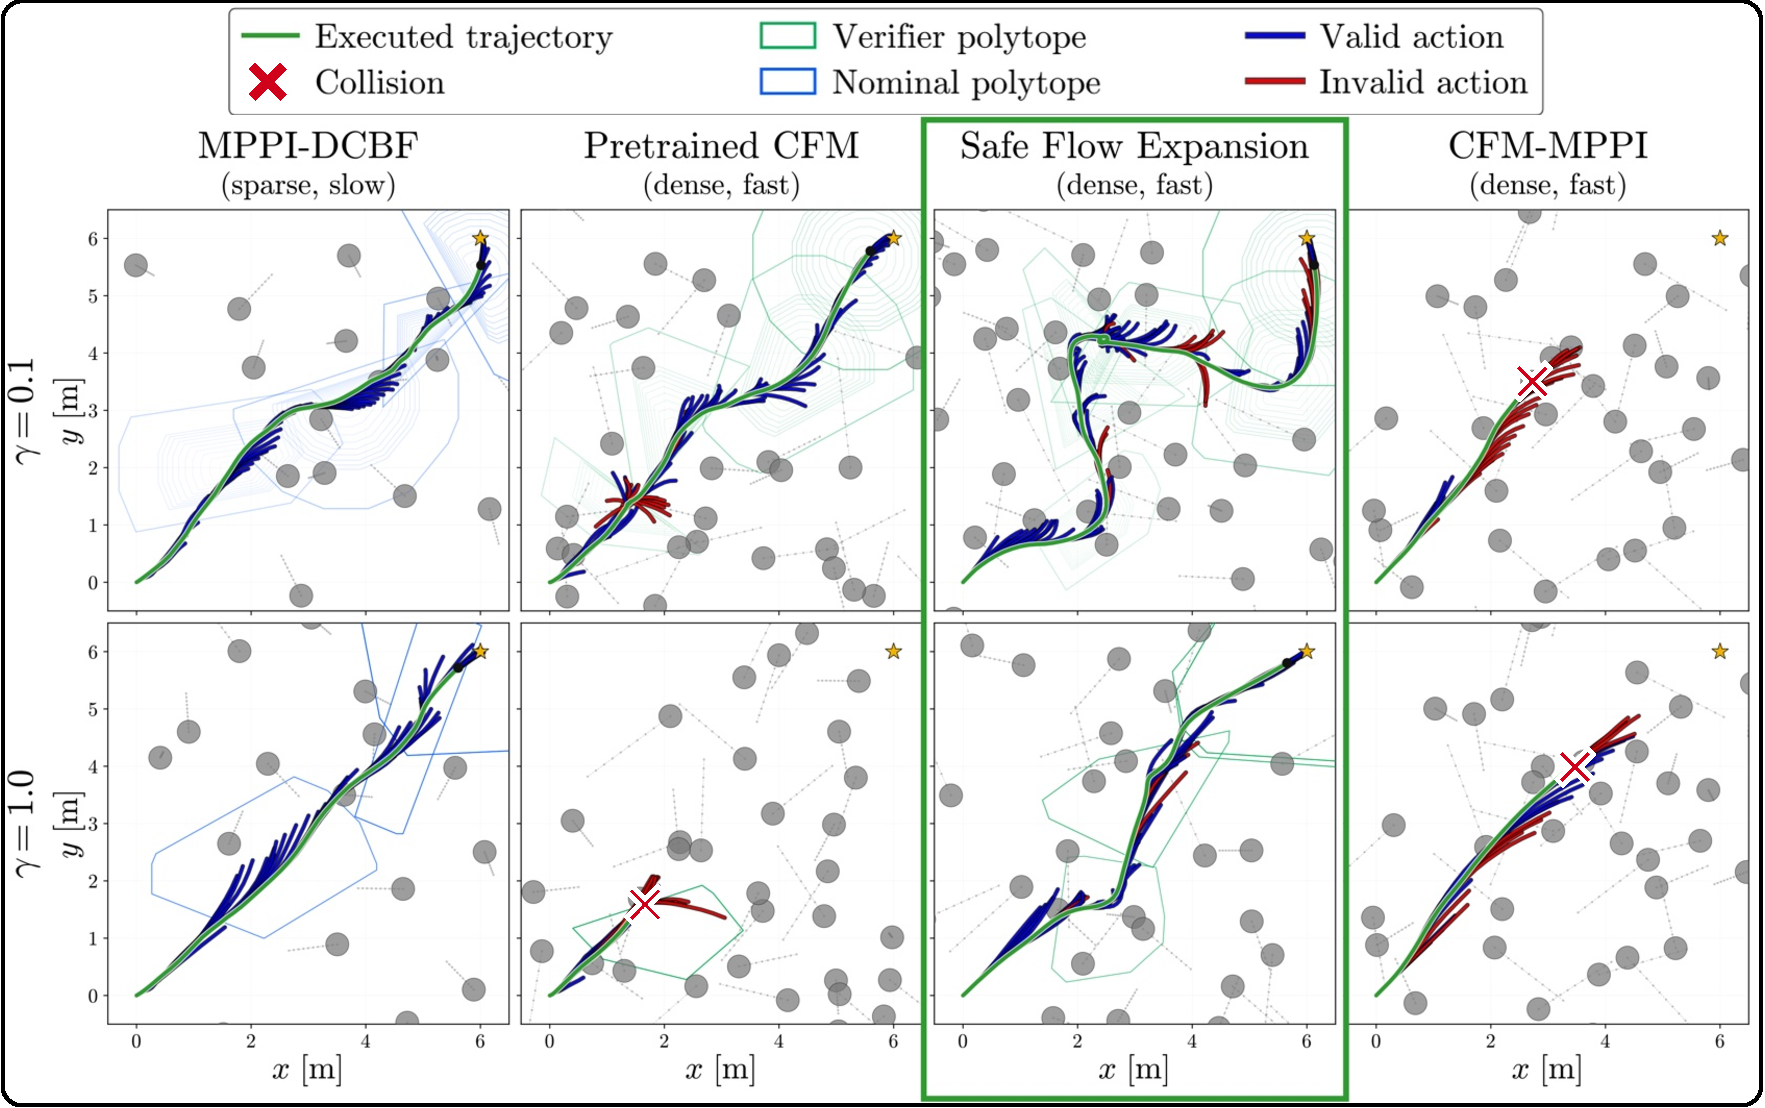
\includegraphics[width=1.0\linewidth]{images/pedestrian_v1_traj-comp.pdf}
    \vspace{-7.0mm}
    \caption{In a challenging dense and fast crowd environment, SFE successfully anticipates and executes valid actions, where $\gamma$ directly controls the valid actions, from conservative behavior ($\gamma=0.1$) to highly aggressive behavior ($\gamma=1.0$).}
\label{fig:pedestrian}
\vspace{-8.0mm}
\end{figure}

\noindent \textbf{Implementation details:} 
The CFM velocity network is one MLP with 3 hidden layers, conditioned on $\gamma$ and the context: the relative goal position, the velocity, and local observation at the current time step $h^\text{poly}$
%(or its 10-step history in the dynamic-pedestrian task) 
within a \(2\mathrm{m}\) sensing range. A convolutional neural network (CNN) downsamples the angular and radial axes of this discretized observation grid and compresses it into a 64-dim observation token. 

At each SFE step, the CFM policy self-generates $K=32$ proposals and resamples $B=16$ of them for verification under~\eqref{eq:importancesampling}, doubled to \((64,32)\) in the dynamic-pedestrian task. Here $K$ controls exploration and $B$ bounds the verification cost. We use the standard MPC cost~\eqref{eq:mppicost} as $C$ to select among valid candidates. Uncertainty is the posterior of an RBF Gaussian process (GP) on the $L_2$-normalized 32-dim $\phi_s$ at flow time $s=0.9$ with a task-specific $\beta$ and length scale calibrated from pretrained embeddings. Also, we use constant-velocity pedestrian predictions in the execution cost to rank valid actions~\cite{mizuta2025unified}, while the verifier certifies actions against the observed geometry held fixed over each horizon.

At deployment, SFE generates one action sequence and executes its first control before replanning. We additionally evaluate cost-based selection among $J>1$ generated sequences in~\Cref{sec:tradeoff}.

\noindent \textbf{Baseline method} We compare against mode-selective CFM-MPPI~\cite{mizuta2025unified}, which combines reward-guided flow generation with local MPPI refinement.  Given a base pre-trained vector field $\mathbf{v}_t^{\theta_{\text{0}}}(\mathbf{x}_t\!\mid\! \mathbf{o},\gamma)$, the guided velocity field is the local gradient ascent of the combined reward
\begin{equation}
   \tilde{\mathbf{v}_t}^{\theta_{\text{0}}}(\mathbf{x}_t\!\mid\! \mathbf{o},\gamma)  = \mathbf{v}_t^{\theta_{\text{0}}}(\mathbf{x}_t\!\mid\! \mathbf{o},\gamma) \;+\; \eta \nabla_{\mathbf{z}_1}R(\mathbf{x},\mathbf{z}_1).
   \label{eq:cfm-mppi_vectorfield}
\end{equation}
The reward combines a CBF-violation penalty and a goal-reaching reward, weighted by $w_\mathrm{s}$ and $w_\mathrm{g}$~\cite[Eq. 6--7]{mizuta2025unified}.

CFM-MPPI generates $J=32$ guided priors at each step, refines the $8$ lowest-cost priors using $M=32$ Gaussian perturbations each, and executes the first control of the lowest-cost refined action. It warm-starts the next replan at flow time $t=0.75$. For each task, we selected the weight pair that best trades off collision rate and time-to-goal.

\subsection{Action Validity across Expansion rounds}
We measure validity as the fraction of executed actions for which \eqref{eq:socp} is feasible for every sensed obstacle, over ten expansion rounds in four OOD environments. Fig.~\ref{fig:validity} shows that expansion increases the average validity relative to the pretrained policy in all four OOD environments. 
This quantitative result supports that Alg.~\ref{alg:sfe} expands the generable set toward valid actions.
The empirical trend across rounds is qualitatively consistent with~\Cref{thm:safe-action-availability} in~\Cref{sec:analysis}.
% TODO: move this 'empirical trend' to analysis section.
% Under the idealized expansion process at a fixed context, the lower bound on the probability that a generated batch contains a valid action is nondecreasing in the number of expansion rounds. 
Also, the higher validity observed at larger $\gamma$ at test time across tasks is consistent with~\Cref{prop:gamma-effect}, as the relaxed verifier condition enlarges the set of actions certified as valid.

\begin{figure}[t]
\centering
    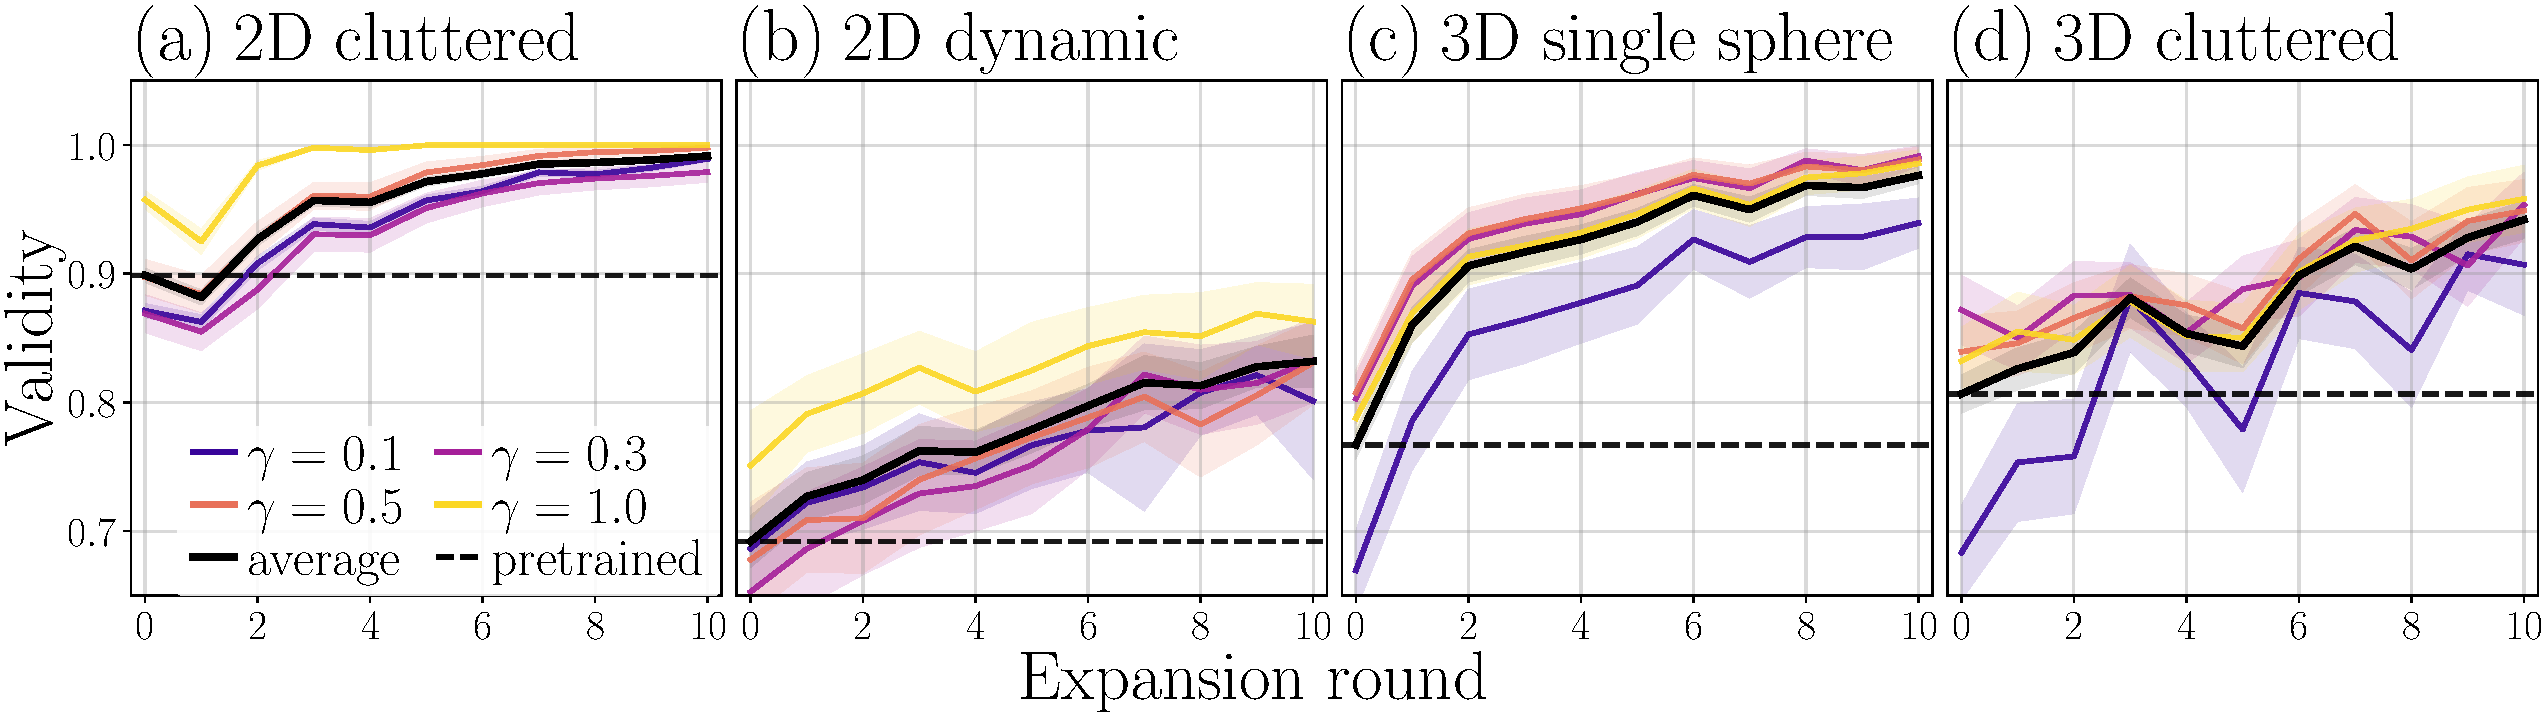
\includegraphics[width=\linewidth]{images/validity_v5.pdf}
    \vspace{-8.0mm}
    \caption{\textbf{Safe Flow Expansion consistently improves validity across four OOD tasks.} Colors denote $\gamma$, black and dashed lines show their average and pretrained average, respectively. Results are acquired over 3 seeds, and 95$\%$ intervals are shown. Expansion and evaluation share OOD configurations in 2D cluttered and 3D single-sphere. The other two tasks use independently sampled OOD configurations unseen during expansion.}
\label{fig:validity}
\vskip -0.25 true in
\end{figure}

Collision rates were 8.3\% for the pretrained CFM, 20.7\% for CFM-MPPI, and 2.3\% for SFE at $\theta_{10}$, across 3 seeds with 100 simulated episodes each in the 3D cluttered task at $\gamma=0.3$. 
Since the finite-horizon DCBF condition \emph{includes} pointwise safety at the first step, the lower collision rates complement the increased validity by showing improved closed-loop safety under receding-horizon execution. 
% TODO Collision rates for other tasks are omitted due to space constraints.
% The adaptation tasks show narrower confidence intervals than the generalization tasks. Adaptation evaluates its 100 test rollouts on one fixed OOD configuration, so variation comes from policy sampling alone. Generalization evaluates independently sampled configurations, which adds variance across configurations. 
%Generalization evaluates independently sampled obstacle configurations, which includes variability from independently sampled obstacle configurations, whereas adaptation is evaluated on a single fixed OOD configuration.

\subsection{Safe Mode Discovery in OOD Environments}

\begin{figure*}[t]
    \centering
    \vspace{-5.0mm}
    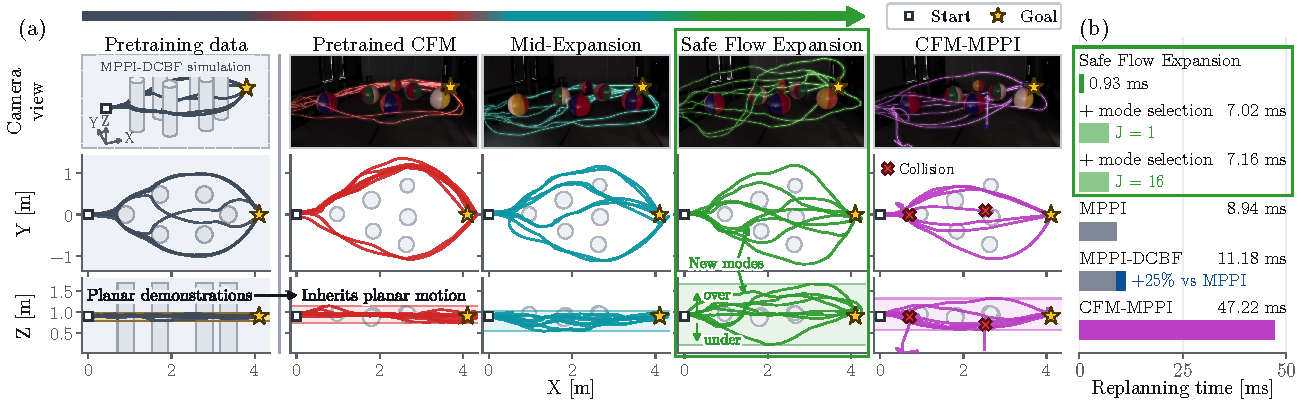
\includegraphics[width=\textwidth]{images/fig_main_side.pdf}
    \vspace{-7.0mm}
    \caption{\textbf{Safe Flow Expansion increases mode coverage in an OOD obstacle geometry at a fraction of the replanning latency of online planners.} Each rollout is assigned a lateral mode according to its binary left/right choice at each gate with \(2^3=8\) possible modes. 
    At checkpoints \(\theta_0\), \(\theta_5\), and \(\theta_{10}\), mode coverage counts the distinct modes observed over 40 random rollouts.
    One representative trajectory is shown for each observed mode. 
    \textbf{(a)} MPPI-DCBF demonstrations among vertical cylinders in simulation, Crazyflie hardware rollouts in one fixed unseen sphere layout for the pretrained CFM, the policy after five expansion rounds, the SFE policy, and CFM-MPPI ($\gamma=0.3$ throughout). 
    \textbf{(b)} Mean per-step replanning time over 100 steps on an NVIDIA RTX 4060 Ti GPU, using 512 rollouts for each MPPI variant and 32 guided proposals for CFM-MPPI.
    }
    \vskip -0.25 true in
    \label{fig:coverage}
\end{figure*}

SFE learns collision-free paths around an unseen large obstacle (Fig.~\ref{fig:2d_cluttered}) and navigates a denser, faster-moving crowd (Fig.~\ref{fig:pedestrian}). 
% TODO explain beyond
In the 3D hardware experiments (Fig.~\ref{fig:coverage}), SFE discovers completely new safe behaviors in OOD beyond those represented in its pretraining demonstrations. 
% TODO (Done) Explained the intuition behind this 'planar lateral' motion generated by MPPI-DCBF.

These demonstrations collected among vertical cylinders are dominated by planar lateral motion, as the MPPI-DCBF assigns low cost to those rollouts under~\eqref{eq:mppicost}. In the unseen cluttered environment with spheres, the pretrained CFM consequently stays close to the demonstration altitude and collapses into two dominant modes. In contrast, SFE covers all eight lateral modes by \(\theta_{10}\) by shifting a probability mass toward fundamentally new safe modes trained offline.

SFE enables this safe mode discovery, but under the tuned $\beta$. The ablation simulation study in Fig.~\ref{fig:beta} shows that $\beta$ controls the balance between exploration and adherence to the prior in the sampling process~\eqref{eq:importancesampling}, under the same verification and policy update procedure. 
Across $3$ seeds, $\beta\!=\!0.1$ recovered all four modes, compared with standard sampling, which covered $2,\!2,\!1$ modes. 
% We demonstrated that SFE not only learns the collision-free path but also discovers completely new safe behaviors in OOD (Fig.~\ref{fig:coverage}).

\subsection{Offline Expansion Cost and Online Planning Latency}
% \subsection{Computation}
\noindent \textbf{Offline expansion.}
Ten rounds of offline expansion took approximately $1$ GPU hour on one NVIDIA H100 NVL GPU in the 3D cluttered task. 
Offline computation cost is dominated by uncertainty-guided self-generation~\eqref{eq:importancesampling}(\emph{$27\%$}) and the verification process~\eqref{eq:socp}(\emph{$24\%$}).
% In a profiled round, the acquisition loop takes $72\%$ of the round, with uncertainty evaluation at \emph{$27\%$} and verification at \emph{$24\%$}. After the loop, \textsc{UpdateBuffer} takes \emph {$ 7\%$}, CFM regression takes \emph{$21\%$}, and \textsc{UpdateUncertainty} (GP refitting) is negligible. 
% Thus, offline computation cost is dominated by uncertainty-guided self-generation~\eqref{eq:importancesampling} and the verification process~\eqref{eq:socp}.
% \textsc{UpdateUncertainty}
% %(line~3)
% , which refits the GP once at the beginning of each round, took negligible time $<0.1\%$. The acquisition loop 
% %(lines~4--14) 
% accounted for $72\%$, where CFM proposal generation 
% %(line~7) 
% used $11\%$, uncertainty evaluation and acquisition in 
% %(line~7) 
% used \emph{$27\%$}, verifier evaluation 
% %(line~8) 
% used \emph{$24\%$}, and rollout $10\%$. After the loop, \textsc{UpdateBuffer} 
% %(line~15) 
% accounted for $7\%$, \textsc{UpdateCFM} regression 
% %(line~16) 
% accounted for $21\%$. 


\noindent \textbf{Online planning.}
\label{sec:compute}
% Safe Flow Expansion (SFE) achieves substantially lower online replanning latency than SBPC and guidance-based CFM, as shown in 
%These reported timings exclude offline training, during which we verify and retrain. Also, the replanning latency scales linearly with the planning horizon, \(\mathcal{O}(H)\).
In Fig.~\ref{fig:coverage}(b), DCBF sample rejection adds only \(2.2\,\mathrm{ms}\) and increases the latency per replan from \(8.9\) to \(11.1\,\mathrm{ms}\) (\(25\%\)). MPPI-DCBF therefore remains practical as an online safety-critical planner while preserving the safety certificate.
CFM-MPPI requires \(47\,\mathrm{ms}\), dominated by online reward-gradient guidance (\(50\%\)) and MPPI refinement (\(40\%\)).
% This sentence is important to stretch the MPPI-DCBF's role as a safety critical planner
With self-generation and verification offline, SFE needs only \(0.93\,\mathrm{ms}\) for one context encoding and unguided flow generation, which is \(12\times\) and \(50\times\) less than MPPI-DCBF and CFM-MPPI.
Cost-based mode selection over \(J\) actions adds a fixed (\(\sim 6\mathrm{ms}\)) overhead from the sequential evaluation induced by velocity clipping. 
SFE still replans faster than both online baselines even at $J=512$.
% However, with parallelized computation, SFE still replans faster than both online baselines even at $J=512$. 
%We therefore used this parallelism to study how \(J\) affects task performance and safety in the following section.
\subsection{Safety-tunable planning and generation via $\gamma$}
\label{sec:tradeoff}
Our framework has the extra benefit of tunable safety through a shared parameter $\gamma$ for online planning~\eqref{eq:poly}, offline verification~\eqref{eq:socp}, and policy conditioning. 
% MPPI-DCBF accepts only rollouts satisfying the bound $(1-\gamma)^i$ in~\eqref{eq:poly} before weighted averaging, with smaller $\gamma$ imposing a stricter safety margin. The verifier applies the same bound in~\eqref{eq:socp}, and Proposition~\ref{prop:gamma-effect} establishes that decreasing $\gamma$ constrains the valid action set. SFE learns this different level of safety and also expands its generable set beyond the demonstrations.
Fig.~\ref{fig:tradeoff} quantitatively shows that $\gamma$ trades off safety and performance in both MPPI-DCBF and SFE. Across both OOD generalization tasks, lower $\gamma$ gives more conservative behavior with greater mean clearance, whereas higher $\gamma$ produces more aggressive behavior with shorter time-to-goal. This can be critical in real-world tasks where the robot must adjust caution to context, as $\gamma$ can serve as a safety knob at deployment.

%TODO stretch SFE overcome the imitation gap
% SFE achieves greater mean clearance than the pretrained CFM under distribution shift. 
With cost-based mode selection ($J=4,16$), SFE achieves even better performance and safety than $J=1$. This benefits from a larger candidate action pool at deployment at the cost of some computational overhead (Fig.~\ref{fig:coverage}(b)).
%Intuitively, a larger batch provides more action candidates for selecting a valid action with low cost.
% as noted in Corollary~\ref{thm:safe-action-availability} although the bound itself does not guarantee improvement of either metric. The following theoretical analysis formally grounds these empirical findings. 
% Across the highly dynamic pedestrian and cluttered 3D OOD environments, SFE achieves greater mean clearance than mode-selective CFM-MPPI~\cite{mizuta2025unified}. These results support that limited coverage of valid behaviors in the pretrained policy, a central motivation for generable-set expansion~\cite{de2026active}, remains a bottleneck for OOD navigation even with online guidance and refinement.
%Thus, the safety parameter lets the robot solve the same task at different safety levels. 
%By contrast, CFM-MPPI varies little across $\gamma$. It guides and refines samples from the same safety-conditioned model, but its guidance reward uses fixed weights $w_\text{s}, w_\text{g}$ and applies neither rejection nor verification.
% The safety and performance difference between MPPI-DCBF and the pretrained policy in Fig.~\ref{fig:tradeoff} is the imitation gap under distribution shift. SFE recovers a broad portion of this gap. 
% In the dynamic-pedestrian task, starting from the same pretrained policy, SFE achieves greater mean clearance and CFM-MPPI instead varies little across $\gamma$, largely maintains the pretrained clearance, and improves primarily in time-to-goal, most visibly in the dynamic pedestrian task. Empirically, increasing $J$ moves SFE toward both higher clearance and lower time-to-goal.
\subsection{Theoretical Analysis of Safe Flow Expansion}
\label{sec:analysis}
This section connects the MPPI-DCBF demonstrations to the initial set for SFE and derives a conditional lower bound on the probability of valid action (See App.~\ref{app:sfe-analysis} for details). 
% TODO: All results apply to a fixed $(\o,\gamma)$, and extending them to online OOD contexts remains future work~\footnote{The following result analyzes an idealized expansion process satisfying Ass.~\ref{assumptions:afe}, while it does not directly characterize the CFM update in Alg.~\ref{alg:sfe}.}.

For a validity threshold $p_{\min}\in(0,1)$ and $\epsilon\in(0,1-p_{\min})$, we denote a measurable $S_0\subseteq\mathcal U^H$ an \textit{initial safe set} if $\operatorname{Vol}(S_0)$ is well defined and positive, $S_0\subseteq\Omega^{\tau}_{\theta_0}(\o,\gamma)\cap\Omega^\star(\o,\gamma)$, and $\inf_{\hat{\mathbf u}\in S_0}\varsigma(\psi(\phi_s(\hat{\mathbf u};\o,\gamma))) \ge p_{\min}+\epsilon$. Let $R_\epsilon$ denote the action-space one-step reachability operator of~\cite[Eq.~(19)]{de2026active}~\footnote{In our notation, this operator maps a set $S\subseteq\mathcal U^H$ of actions to \(R_\epsilon(S)\!:=\!\{\hat{\mathbf u}\in\mathcal U^H\!:\!\!\!\ \exists\,\hat{\mathbf u}'\!\in\! S\ \text{s.t.}\;\varsigma(\psi(\phi_s(\hat{\mathbf u}'\!;\o,\!\gamma)\!)\!)\!-\!L_\varsigma L_\psi\,d(\hat{\mathbf u},\!\hat{\mathbf u}')\!-\!\epsilon\ \!\!\ge\!p_{\min}\},\) where $d(\hat{\mathbf u},\hat{\mathbf u}'):=\|\phi_s(\hat{\mathbf u};\o,\gamma)-\phi_s(\hat{\mathbf u}';\o,\gamma)\|_2$ is the feature distance, and $L_\varsigma$ and $L_\psi$ are the Lipschitz constants of $\varsigma$ and $\psi$ in the analysis model.} with $\mathcal X=\mathcal U^H$ and $\phi=\phi_s(\cdot;\o,\gamma)$. We use  $R_\epsilon^r$ for $r$ repeated applications of this operator.

The MPPI-DCBF demonstrations provide only finitely many valid actions as in Prop.~\ref{prop:nominal-verifier}, which by themselves have zero volume in the action space and therefore cannot form the initial set required by the expansion analysis.
The following lemma uses strict feasibility and continuity to extend these actions to neighborhoods of positive volume.
% The MPPI-DCBF demonstrations provide only finitely many verified actions as in Prop.~\ref{prop:nominal-verifier}, which by themselves have zero volume in the action space and therefore cannot form the initial set required by the expansion analysis. The following lemma bridges this gap by enlarging each verified action into a small safe neighborhood, whose union provides a nonzero-volume initial safe set for SFE.
% strict feasibility and continuity 
\begin{lemma}[Initial safe set from MPPI-DCBF]
\label{lem:seed}
Under the conditions of Proposition~\ref{prop:nominal-verifier}, let $Q\ge1$ and let $\{\hat{\mathbf u}_0^{(q)}\}_{q=1}^{Q}\subset\operatorname{int}(\mathcal U^H)$ be a finite set of MPPI-DCBF actions satisfying~\eqref{eq:poly} strictly with $h=h^{\mathrm{poly}}$, with $p_1^{\theta_0}(\hat{\mathbf u}_0^{(q)}\mid\o,\gamma)>\tau$ and $\varsigma(\psi(\phi_s(\hat{\mathbf u}_0^{(q)};\o,\gamma)))>p_{\min}+\epsilon$. 
If the dynamics in~\eqref{eq:dynamical_system} are continuous in the state and action,
% If the resulting finite-horizon trajectory depends continuously on $\hat{\mathbf u}$ at these actions, 
and
$p_1^{\theta_0}(\cdot\mid\o,\gamma)$ and $\varsigma\circ \psi\circ\phi_s$ are
continuous, then there exist radii $\rho_q>0$ such that
$S_0:=\bigcup_q B_{\rho_q}(\hat{\mathbf u}_0^{(q)})$ is an initial safe set, where \(B_\rho(\bar{\mathbf u})\) denotes the open Euclidean ball \(\left\{\hat{\mathbf u}\!\in\!\mathcal U^H\!:\!\|\hat{\mathbf u}\!-\!\bar{\mathbf u}\|_2\!<\!\rho\right\}\).
\end{lemma}

\begin{proof}
The predicted states depend continuously on $\hat{\mathbf u}$. Thus, all strict inequalities remain satisfied in a sufficiently small ball around each $\hat{\mathbf u}_0^{(q)}$ contained in $\mathcal U^H$. By Proposition~\ref{prop:nominal-verifier}, these balls contain only valid actions. Their union has positive volume and satisfies the density and validity-score conditions, hence forms an initial safe set.\hfill$\blacksquare$
% By continuity of the dynamics in~\eqref{eq:affinesystem}, the induced finite-horizon trajectory map is continuous in $\hat{\mathbf u}$. 
% Since all relevant conditions are strict, they remain true for actions sufficiently close to each $\hat{\mathbf u}_0^{(q)}$. Choose each $\rho_q$ small enough that its ball remains inside $\mathcal U^H$ and preserves these conditions. \Cref{prop:nominal-verifier} then places every such ball in $\Omega^\star(\o,\gamma)$.
\end{proof}

With the initial safe set $S_0$ provided under the conditions of Lemma~\ref{lem:seed}, Lemma~\ref{lem:coverage} guarantees the \emph{coverage event}~\eqref{eq:coverage} after $T^\star\!=\!rT$ sequential queries and model updates of the idealized process at a fixed $(\o,\gamma)$.
Specifically, \(\Pr(\mathcal E_{\mathrm{cov}})\!\ge\!1\!-\!\delta\). This gives the following sampling guarantee.
% Lemma~\ref{lem:seed} requires a finite set of actions that satisfies the strict conditions and remains valid under sufficiently small action changes. Starting from this initial safe set $S_0$, Lemma~\ref{lem:coverage} guarantees that after $T^\star=rT$ sequential query of model updates at a fixed $(\o,\gamma)$ after which the coverage event $\mathcal E_{\mathrm{cov}}\!:=\!\{R_\epsilon^r(S_0)\!\subseteq\!\Omega_{\theta_{T^\star}}^\tau\!(\o,\gamma)\}$ holds with probability at least $1-\delta$, \textit{i.e.,} $\Pr(\mathcal E_{\mathrm{cov}})\ge1-\delta$. This gives the following sampling guarantee.
\begin{corollary}[Probability of valid action after expansion]
\label{thm:safe-action-availability}
Under the setting above, let $r\!\ge\!1$ be an integer and define
$\mathcal A_{\gamma,r}(\o)\!:=\!R_\epsilon^r(S_0)\cap\Omega^\star(\o,\gamma)$
and $m_{\gamma,r}(\o):=\operatorname{Vol}(\mathcal A_{\gamma,r}(\o))$. Then $m_{\gamma,r}(\o)\ge\operatorname{Vol}(S_0)>0$, and $m_{\gamma,r}(\o)$ is nondecreasing in $r$. 
Given the expansion history,
independently sample $J\ge1$ actions from $p_1^{\theta_{T^\star}}(\cdot\mid\o,\gamma)$, we obtain
\begin{equation}
\Pr\!\left[\exists\,\!j\!\le\! J\!:\! v_\gamma(\hat{\mathbf u}^{(j)};\!\o)\!=\!1\right]
% &\!\ge\!
% (1-\delta)\!\left[1-\!\bigl(1\!-\!\tau m_{\gamma,r}(\o)\!\bigr)^{J}\right]\!\\
\!\ge\!
(1-\delta)\!\left[1\!-\!e^{\!-J\tau m_{\gamma,r}(\o)}\right]\!\!.
\label{eq:main1}
\end{equation}
\end{corollary}
\begin{proof}
By definition of the reachability operator
\(S_0\!\subseteq\!R_\epsilon^r(S_0)\!\subseteq\! R_\epsilon^{r+1}(S_0)\). Intersecting with $\Omega^\star(\o,\gamma)\supseteq S_0$ gives $\operatorname{Vol}(S_0)\le m_{\gamma,r}(\o)\le m_{\gamma,r+1}(\o)$. On the coverage event $\mathcal E_{\mathrm{cov}}$~\eqref{eq:coverage}, every action in $\mathcal A_{\gamma,r}(\o)$ is valid and has density at least $\tau$. Then, by the independence of the $J$ sample, we get the conditional bound \(1\!-\!\left(1\!-\!\tau m_{\gamma,r}(\o)\right)^J\). Applying \(1\!-\!x\!\le \!e^{-x}\) and $\Pr(\mathcal E_{\mathrm{cov}})\ge1-\delta$ gives~\eqref{eq:main1}.\hfill$\blacksquare$
\end{proof}
For fixed $(\o,\gamma,S_0,\epsilon,\tau,\delta)$, the lower bound in~\eqref{eq:main1} is nondecreasing in both reachability depth $r$ and batch size $J$. Corollary~\ref{thm:safe-action-availability} provides a valid action sampling guarantee for an idealized expansion process, while improvements, such as validity improvement in rounds (Fig.~\ref{fig:validity}) and the higher clearance and shorter time-to-goal with larger $J$ (Fig.~\ref{fig:tradeoff}), under the implemented Alg.~\ref{alg:sfe} are established empirically. 
% ~\footnote{This conclusion neither assumes that the conditional generable set for one $r$ is contained in the next nor uses the same coverage condition for different $r$. The claim applies only to the guaranteed lower bound, and it does not claim that the validity of each later CFM policy must increase.}.
% Proposition~\ref{prop:gamma-effect} establishes an inclusion between valid action sets $\Omega^\star(\o,\gamma)$ at different values of $\gamma$, whereas Corollary~\ref{thm:safe-action-availability} applies separately to each fixed $(\o,\gamma)$~\footnote{Changing $\gamma$ may also change the conditional policy, learned representation, initial safe set, and reachability operator.}.
% Therefore, Prop.~\ref{prop:gamma-effect} does not imply an inclusion between the corresponding reachable or conditional generable sets, and hence does not imply monotonicity of $m_{\gamma,r}(\o)$ or~\eqref{eq:main1} in $\gamma$.
% The lower bound in~\eqref{eq:main1} is nondecreasing with $r$ as $m_{\gamma,r}(\o)$ is nondecreasing by the monotonicity of the reachability operator, for fixed $(\o,\gamma,S_0,\epsilon,\tau,\delta,J)$~\footnote{This conclusion neither assumes that the conditional generable set for one $r$ is contained in the next nor uses the same coverage condition for different $r$. The claim applies only to the guaranteed lower bound, and it does not claim that the validity of each later CFM policy must increase.}. Also, not only the effect of $r$ but also the effect of $\gamma$ can be noted. Proposition~\ref{prop:gamma-effect} establishes an inclusion between valid action sets $\Omega^\star(\o,\gamma)$ at different values of $\gamma$, whereas Corollary~\ref{thm:safe-action-availability} applies separately to each fixed $(\o,\gamma)$~\footnote{Changing $\gamma$ may also change the conditional policy, learned representation, initial safe set, and reachability operator.}. Therefore, Proposition~\ref{prop:gamma-effect} by itself does not imply an inclusion between the corresponding reachable or conditional generable sets, and hence does not imply monotonicity of $m_{\gamma,r}(\o)$ or~\eqref{eq:main1} in $\gamma$.
\begin{figure}[t]
    \centering
    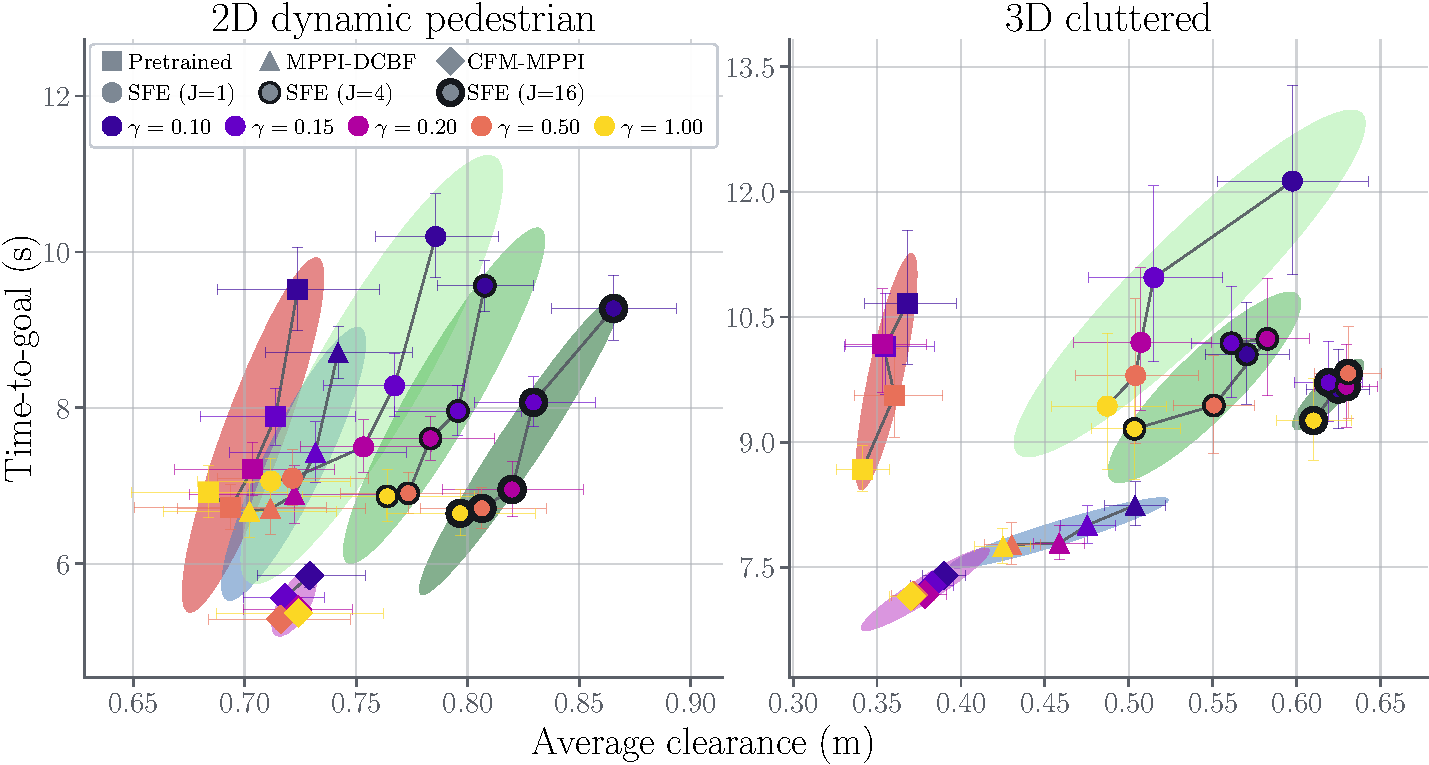
\includegraphics[width=\linewidth]{images/tradeoff_v2.pdf}
    % TODO change it to .pdf before submission:)
    \vspace{-8.0mm}
    \caption{\textbf{Safety--performance trade-off under a shared safety parameter $\gamma$.} Two OOD generalization tasks compare the pretrained CFM, MPPI-DCBF, CFM-MPPI, and SFE at different values of $\gamma$ and $J$ (SFE).
    % Across both tasks, $\gamma$ modulates behavior from conservative to aggressive for MPPI-DCBF and SFE.
    Results are acquired over 3 seeds, 95$\%$ intervals are shown, and lines connect increasing $\gamma$ within each method.
    %, where CFM-MPPI barely moves, and larger $J$ empirically shifts SFE toward higher clearance and lower time to goal.
    }
    \label{fig:tradeoff}
    \vskip -0.25 true in 
\end{figure}
\section{Conclusion}

We presented a unified safe sampling-based planning paradigm. MPPI-DCBF certifies safety after MPPI's weighted averaging with modest computational overhead. Safe Flow Expansion uses offline computation to expand the generable set of CFM policies toward valid behaviors, enabling new safe modes in OOD environments. A shared safety parameter $\gamma$ specifies the finite-horizon DCBF conditions and tunes the conservativeness of both the online planner and generative policy.

Future work will study conditions for recursive feasibility of MPPI-DCBF under finite sampling, combine expanded CFM policies with lightweight run-time safety filters to provide hard safety guarantees, and learning an optimal $\gamma$ schedule directly from data remains an interesting open problem. 
Our concrete next step is to scale the offline SFE framework to systems where expert demonstrations are prohibitively expensive, such as safety-critical manipulation, building on the preliminary results in Fig.~\ref{fig:robotarm}.

% Under the assumptions of~\Cref{sec:analysis}, Corollary~\ref{thm:safe-action-availability} lower bounds the probability that a generated batch contains a valid action at a fixed context and $\gamma$.

% We presented a unified sampling-based planning paradigm that addresses unsafe averaging in model predictive path integral control (MPPI) and limited coverage of safe behaviors in conditional flow matching (CFM) policy in out-of-distribution (OOD). Our approach used a finite-horizon DCBF condition for multi-step safe online planning and generative policy. Hardware and simulation experiments show that offline Safe Flow Expansion (SFE) improves validity over the pretrained policy and discovers new modes absent from demonstrations, across tested OOD environments.

% Future work could combine our expanded CFM policy with a lightweight run-time safety filter to provide hard guarantees. Also, learning an optimal $\gamma$ schedule directly from data remains an interesting open problem. Such dynamic scheduling would allow the system to tightly trade off safety and performance.
% Our next step is to scale the offline SFE framework to systems where expert demonstrations are prohibitively expensive, such as safety-critical manipulation, building on the preliminary results in Fig.~\ref{fig:robotarm}.
% Safe Flow Expansion raises verifier validity over the pretrained policy in four OOD environments and discovers new modes absent from the demonstrations. With self-generation and verification offline, the expanded policy replans at a fraction of the baseline methods. We also demonstrated that the safety parameter $\gamma$ tunes both the online planner and the expanded policy along a clearance/time-to-goal frontier.
% Learning an optimal $\gamma$ schedule directly from data remains an interesting open problem (\textit{e.g.,} rather than a fixed $\gamma$ during deployment). Such dynamic scheduling would allow the system to tightly trade off safety and performance, which can be critical in real-world tasks where the robot must adjust caution to context.
% Under the assumptions of~\Cref{sec:analysis}, Corollary~\ref{thm:safe-action-availability} provides lower bounds, with high probability, at a fixed context and $\gamma$, on the probability that a generated batch contains a valid action. Future work could explore combining our expanded policy with a lightweight run-time safety filter to provide hard guarantees. Our next step is to extend SFE to safety-critical manipulation, where expert demonstrations are costly, building on the preliminary MPPI-DCBF results in Fig.~\ref{fig:robotarm}.

\textbf{Acknowledgments} Claude Opus 5 was used as an aid to develop helper functions in the code and LaTeX formatting.
% Our next step is to scale the framework to systems with extremely large state spaces or where expert demonstrations are prohibitively expensive. In parallel, while our method robustly expands the safe action distribution, tuning the online execution cost $C$ can still shift the distribution away from the prior actions, which remains an important challenge.
\bibliographystyle{IEEEtran}
\bibliography{references}
\section{Appendix: Analysis Details for SFE}
\label{app:sfe-analysis}
We state the conditions of~\cite[Thm.~F.5]{de2026active} directly on $\mathcal U^H$ using the frozen kernel
% We apply the generable set expansion analysis of~\cite{de2026active} directly in the SFE action space. The cited theorem is written in a learned representation space, whereas our verifier~\eqref{eq:verifier-certified-set} and conditional generable set~\eqref{eq:conditional-generable-set} are defined on $\mathcal U^H$. We therefore state its conditions on $\mathcal U^H$ and use the representation only through the frozen kernel
\begin{equation}
k_{\phi}^{\o,\gamma}(\hat{\mathbf u},\hat{\mathbf u}')
:=k(\phi_s(\hat{\mathbf u};\o,\gamma),\phi_s(\hat{\mathbf u}';\o,\gamma)).
\end{equation}
% The verifier $v_\gamma$ is deterministic. Thus, the random variable $Y$ below is used only by the probabilistic model in the analysis which is not the verifier output. Deterministic validity is imposed separately through the common set with $\Omega^\star(\o,\gamma)$.
The auxiliary observation $Y$ in Assumption~\ref{assumptions:afe} is distinct from the deterministic labels produced by $v_\gamma$.
\begin{assumption}[Analysis model, {\cite[App.~F]{de2026active}}]
\label{assumptions:afe}
Fix $(\o,\gamma)$ and a validity threshold $p_{\min}\in(0,1)$.
(i) The auxiliary binary observation follows the RKHS logistic model $\Pr[Y=1\mid\hat{\mathbf u}]=\varsigma(\psi(\phi_s(\hat{\mathbf u};\o,\gamma)))$, for which anytime confidence sequences exist~\cite{pasztor2024bandits}, with $\varsigma$ the $L_\varsigma$-Lipschitz sigmoid, $\psi\circ\phi_s(\cdot;\o,\gamma)\in\mathcal H_{k_\phi^{\o,\gamma}}$, $\|\psi\circ\phi_s(\cdot;\o,\gamma)\|_{k_\phi^{\o,\gamma}}\le B_g$, $\psi$ is $L_\psi$-Lipschitz in a metric $d$, and $\phi_s$ frozen over the query sequence.
(ii) Queried actions lie in a compact subset of $\mathcal U^H$ on which
$k_\phi^{\o,\gamma}\le1$.
(iii) Each CFM update uses the energy-based model update described
in~\cite{de2026active}. Within the current conditional generable set, the uncertainty-tilted sampler in~\eqref{eq:importancesampling} selects an action that approximately maximizes $\sigma_n$.
\end{assumption}

\begin{lemma}[Restatement {\cite[Thm.~F.5]{de2026active}} in $\mathcal U^H$]
\label{lem:coverage}
Fix $\delta\in(0,1)$, $\epsilon\in(0,1-p_{\min})$, a positive integer $r$, and a seed $S_0$.
Assume every condition of~\cite[Thm.~F.5]{de2026active} after replacing its state set with $\mathcal U^H$ and feature map by $\phi_s(\cdot;\o,\gamma)$~\footnote{This includes the conditions on the energy-based model, density threshold, calibration, oracle, sample-complexity conditions, and auxiliary radius.}.
For fixed $(\o,\gamma)$, there exists $T^\star=rT$ such that the coverage event
\begin{equation}
\label{eq:coverage}
\mathcal E_{\mathrm{cov}}
:=
\left\{
R_\epsilon^r(S_0)
\subseteq
\Omega_{\theta_{T^\star}}^\tau(\o,\gamma)
\right\}
\end{equation}
satisfies
$\Pr(\mathcal E_{\mathrm{cov}})\ge1-\delta$.
\end{lemma}
% Alg.~\ref{alg:sfe} uses batched acquisition and updates across contexts, so its total verifier count is distinct from this analysis budget.
Alg.~\ref{alg:sfe} queries the verifier in batches and updates the policy using data from multiple contexts.
Its total number of verifier calls therefore does not directly correspond to $T^\star$.
% Here $T^\star$ is the number of sequential query and model update steps performed at $(\o,\gamma)$. In practice, Alg.~\ref{alg:sfe} freezes $\theta_n$ and $\sigma_n$ within a batch and combines data from different contexts. Therefore, we cannot use its total number of verifier evaluations directly as $T^\star$. Combining data from different contexts does not change the definitions of $\mathcal A_{\gamma,r}(\o)$ or $m_{\gamma,r}(\o)$. However, the probability $1-\delta$ applies separately to each context. During SFE acquisition, $v_\gamma$ evaluates every candidate action before cost-based execution. 
\end{document}